% !TeX program = lualatex
\documentclass[12pt, a4paper]{article}

% ==========================================
% 中文 review 版：内容对应 Report/main.tex
% ==========================================
\usepackage{fontspec}
\setmainfont[ItalicFont={Noto Sans CJK SC}]{Noto Sans CJK SC}
\setsansfont[ItalicFont={Noto Sans CJK SC}]{Noto Sans CJK SC}
\setmonofont{Latin Modern Mono}
\usepackage[left=2.5cm, right=2.5cm, top=2.5cm, bottom=2.5cm]{geometry}
\usepackage{setspace}
\onehalfspacing
\raggedright
\setlength{\parindent}{0pt}
\setlength{\parskip}{0.45em}
\emergencystretch=3em
\directlua{
local glyph = node.id("glyph")
local penalty = node.id("penalty")
local function is_cjk(c)
  return (c >= 0x2E80 and c <= 0x9FFF)
      or (c >= 0xF900 and c <= 0xFAFF)
      or (c >= 0xFE10 and c <= 0xFE6F)
      or (c >= 0xFF00 and c <= 0xFFEF)
end
local function add_cjk_breaks(head)
  local n = head
  while n do
    if n.id == glyph and is_cjk(n.char) then
      local p = node.new(penalty)
      p.penalty = 0
      head = node.insert_after(head, n, p)
      n = p.next
    else
      n = n.next
    end
  end
  return head
end
if luatexbase and luatexbase.add_to_callback then
  luatexbase.add_to_callback("pre_linebreak_filter", add_cjk_breaks, "mainzh_cjk_breaks")
else
  callback.register("pre_linebreak_filter", add_cjk_breaks)
end
}

% ==========================================
% Packages
% ==========================================
\usepackage{graphicx}
\graphicspath{{figures/}}
\usepackage{float}
\usepackage{placeins}
\usepackage[font=small,labelfont=bf,labelsep=period]{caption}
\usepackage{subcaption}
\usepackage{booktabs}
\usepackage{longtable}
\usepackage{array}
\usepackage{ragged2e}
\usepackage{siunitx}
\usepackage{tikz}
\usetikzlibrary{arrows.meta,positioning,calc,fit,shapes.geometric}
\usepackage{titlesec}
\titlespacing*{\section}{0pt}{1.1em}{0.45em}
\titlespacing*{\subsection}{0pt}{0.9em}{0.35em}
\usepackage{xurl}
\usepackage{chngcntr}
\counterwithin{figure}{section}
\counterwithin{table}{section}
\captionsetup[figure]{name=图}
\captionsetup[table]{name=表}
\usepackage[backend=biber, style=ieee]{biblatex}
\addbibresource{references.bib}
\defbibheading{bibliography}{\section*{参考文献}}
\usepackage[pdfpagelabels]{hyperref}
\hypersetup{
    pdftitle={B-BOT Chinese Review Copy},
    pdfauthor={Botao Su},
    pdfsubject={Chinese review copy of the B-BOT final report}
}
\renewcommand{\theHfigure}{\thesection.\arabic{figure}}
\renewcommand{\theHtable}{\thesection.\arabic{table}}
\tikzset{
    diagramblock/.style={draw, rounded corners=2pt, align=center, font=\scriptsize, minimum height=0.72cm, text width=2.8cm},
    diagramsmall/.style={draw, rounded corners=2pt, align=center, font=\scriptsize, minimum height=0.62cm, text width=2.35cm},
    diagramstate/.style={draw, rounded corners=2pt, align=center, font=\scriptsize, minimum height=0.68cm, text width=2.25cm},
    diagramarrow/.style={-{Stealth[length=2mm]}, thick},
    diagramnote/.style={align=center, font=\scriptsize}
}
\newif\ifplanningphysicaldata
\planningphysicaldatafalse
\newcommand{\planningCaptionSuffix}{\ifplanningphysicaldata （planning data）\fi}
\newcommand{\planningDataNote}[1]{\ifplanningphysicaldata #1\fi}

\begin{document}
\hypersetup{pageanchor=false}

\begin{titlepage}
    \centering
    \vspace*{2cm}
    {\fontsize{24pt}{28pt}\selectfont \textbf{B-BOT：带 ROS 2 视觉遥操作的 WiFi 自平衡轮腿机器人}\par}
    \vspace{2cm}
    {\Large \textbf{三年级个人项目 -- 最终报告}\par}
    \vspace{1cm}
    {\large 2026 年 5 月\par}
    \vspace{3cm}
    {\large \textbf{Botao Su}\par}
    \vspace{0.5cm}
    {\large 学生识别号：\textbf{1107124}\par}
    \vspace{3cm}
    {\large 指导教师：\textbf{Dr Liam Marsh}\par}
    \vfill
\end{titlepage}
\hypersetup{pageanchor=true}
\pagenumbering{roman}

\newpage
\section*{摘要}
B-BOT 是一台自平衡轮腿机器人。本项目用它研究如何把实时嵌入式平衡控制与安全的无线遥操作和视觉遥操作结合起来。与传统双轮自平衡机器人相比，轮腿机器人能够改变机身高度，并协调轮子和腿部运动，因此具备更高的运动能力；但这也增强了机身俯仰、轮端力矩和腿部几何之间的耦合。 因此，本项目的核心设计约束是：稳定反馈必须保留在嵌入式控制器本地，不能依赖 WiFi、摄像头处理或主机端软件时序。

已实现的系统使用 ESP32 控制器运行 FreeRTOS 任务，完成电机反馈、惯性测量、腿部运动学、目标更新和平衡控制。平衡控制器结合线性二次型调节器（LQR）实现矢状面平衡，使用 PID 环控制偏航、横滚和腿长，并通过虚拟模型控制（VMC）把虚拟腿部力和力矩映射为关节电机指令。主机端 ROS 2 视觉桥接节点从 ROS 2 WiFi 摄像头模块接收图像，运行基于 MediaPipe 的感知，并通过 WiFi TCP 文本协议向机器人发送监督级命令。Xbox BLE、UART 命令、WiFi TCP 命令和视觉生成命令通过共享命令解析、队列逻辑、看门狗和安全门控进行协调。

系统评估包括控制环抖动、WiFi 命令进入延迟、看门狗故障注入、摄像头启动、视觉命令延迟和实时手势识别测试\planningDataNote{；静态平衡、扰动恢复、腿长敏感性、物理遥操作响应和控制器消融目前作为待最终硬件采集的数据结构保留}。比较性 baseline 测试用于评估额外的控制器复杂度是否得到合理证明。实测控制环日志在 15000 个样本上显示平均周期为 3.9998 ms，中位周期为 4.000 ms。WiFi TCP 命令进入测试在 300 个样本中取得 37.41 ms 的 ACK 中位延迟和 88.31 ms 的 p95 延迟，且无未匹配命令。看门狗故障注入测试在 10 次直接命令看门狗试验中全部清除命令，检测到全部 10 次 TCP 关闭试验，并在全部 10 次空闲试验中产生 full-stop 事件。实时视觉测试得到干净的 6/6 命令类别矩阵、85.3\% 的选中帧标签准确率，以及 71 条安全命令上的 66.13 ms 桥接到 ESP32 ACK 中位延迟。主要限制是视觉和 WiFi 层只适合监督级遥操作，不适合闭合稳定控制环。本项目贡献是一套实用的嵌入式轮腿平衡架构，并在其上扩展了具有安全意识的多源命令仲裁和 ROS 2 视觉遥操作。

\newpage
\section*{原创性声明}
我确认本 dissertation 是我自己的原创工作，除非文中明确引用或说明为其他来源。来自其他来源的文字、图、代码、数据和思想均已在报告、参考文献或附录中按需要注明。

\newpage
\section*{知识产权声明}
本 thesis 的作者拥有其中某些版权或相关权利。项目所使用的第三方代码、库和厂商材料已在软件附录和参考文献中标识。

\newpage
\tableofcontents

\newpage
\listoffigures
\listoftables

\newpage
\pagenumbering{arabic}
\section{引言}

\subsection{背景与动机}

自平衡机器人是有价值的工程平台，因为它在一个紧凑系统中结合了不稳定动力学、嵌入式传感、实时控制和执行器协调。传统双轮自平衡机器人主要通过轮端力矩在移动时调节机身俯仰。轮腿机器人在此基础上增加可控腿部几何，使机身高度、支撑力和动态姿态可以被改变。这提升了机动性，但也使控制问题更困难，因为机身俯仰、轮子运动、腿长和关节力矩之间出现强耦合。

本项目开发了 B-BOT，一台基于 ESP32 嵌入式控制器的 WiFi 自平衡轮腿机器人。主要工程问题并不只是让机器人站起来。更困难的问题是，把实时嵌入式平衡控制与多个非实时命令源集成，同时不允许这些命令源使机器人失稳。B-BOT 可以接收 Xbox BLE 控制器、UART 脚本命令、主机电脑 WiFi TCP 命令，以及 ROS 2 / MediaPipe 视觉桥接命令。这些输入最终作用于同一台物理机器人，因此系统必须避免命令冲突，并且在某个命令源消失时安全失效。

核心设计决策是把稳定控制环保留在 ESP32 本地。俯仰、轮子和腿部反馈在嵌入式控制器上处理，LQR/PID/VMC 控制计算在 FreeRTOS 任务中执行。主机端软件被刻意排除在平衡环之外。这是必要的，因为 WiFi 延迟、摄像头帧率、ROS 2 调度和 MediaPipe 推理都无法在平衡控制器目标的 4 ms 时间尺度上保持确定性。

因此，本项目中的 ROS 2 部分被用作监督级感知层，而不是底层控制总线。ROS 2 WiFi 摄像头模块通过模块侧 micro-ROS 图像传输把图像提供给主机 ROS 2 系统。主机端 \texttt{\detokenize{wheeleg_vision_bridge}} 处理这些图像，并把识别出的视觉事件转换为文本命令。随后这些命令通过 WiFi TCP 文本协议发送到 ESP32。在当前实现中，底层 ESP32 机器人控制器不是 micro-ROS 节点。

这种架构的动机是实际安全性。视觉遥操作对演示和人机交互有用，但一次错误的手势分类或网络延迟不应直接使机器人失稳。通过把视觉和 WiFi 命令视为带有看门狗过期机制的临时目标请求，B-BOT 以可控、可测试的方式把本地实时平衡控制与高层远程输入结合起来。因此，本项目贡献是一种集成的安全感知嵌入式机器人架构，而不是宣称视觉或 WiFi 适合闭合稳定反馈环。

\subsection{目标与任务}

本项目的总体目标是设计、实现并评估一台自平衡轮腿机器人，使其把实时嵌入式平衡控制与安全的无线和视觉监督级遥操作结合起来。

项目任务如下：

\textbf{O1 — 嵌入式轮腿平衡控制。}
开发基于 ESP32 的控制系统，结合 LQR、PID 环和 VMC 来稳定机器人、调节腿部几何，并输出轮子/关节力矩。该任务通过静态平衡、扰动恢复、腿长变化、遥操作阶跃响应和控制环抖动测试进行评估。

\textbf{O2 — ROS 2 视觉输入与 WiFi TCP 命令通道。}
实现主机端 ROS 2 视觉流水线和 WiFi TCP 命令路径，使其能够生成并传输监督级机器人命令，同时不进入稳定反馈环。该任务通过 TCP 命令进入延迟、摄像头话题检查、视觉桥接 ACK 延迟和实时手势识别测试进行评估。

\textbf{O3 — 安全的多源输入仲裁。}
支持 Xbox BLE、UART 脚本命令、WiFi TCP 命令和视觉生成命令，同时避免不同输入源之间产生不受控冲突。该任务通过命令队列行为、直接命令看门狗、TCP 断开/空闲故障注入、\texttt{\detokenize{dry_run}} 视觉测试、stunt arming 行为和停止命令验证进行评估。

成功标准不以最大速度或完全自主导航为核心。相反，本项目通过机器人是否展示了稳定的嵌入式平衡、可预测的命令处理，以及在真实通信和感知故障下基于证据的安全行为来判断。

\subsection{报告结构}

第 2 章回顾双轮和轮腿自平衡机器人、不稳定移动机器人的控制策略，以及非确定性网络中的 ROS 2 / micro-ROS 通信。该章用于识别支撑所选架构的技术缺口。第 3 章介绍已实现的系统设计，包括硬件集成、嵌入式任务结构、传感、状态估计、控制算法、WiFi TCP 通信和输入仲裁。第 4 章通过直接对应三个任务的实验评估系统。第 5 章总结技术贡献、限制和未来工作。

\subsection{项目管理}

本项目以迭代式工程构建方式管理，而不是一次性线性实施。初始计划把工作分为硬件 bring-up、嵌入式控制、通信集成、主机端视觉、测试和最终报告。附录 B 包含项目计划和甘特图，包括报告写作阶段使用的最终进度。与原计划相比，主要偏差是底层平衡控制和安全处理比预期需要更多时间，而 ROS 2 视觉层必须收敛为监督级遥操作功能，而不是稳定控制环的一部分。

风险管理分为两部分。第一，附录 E 的健康与安全风险评估覆盖学生和其他人在实际工作中的风险，包括高力矩运动关节、自平衡机器人跌倒、焊接烫伤和烟雾、电池和接线故障、尖锐打印件或加工件、拖曳线缆，以及无线或视觉测试中的意外运动。这些风险通过适合实验室的监督工作方式、自由站立测试前的低能量台架测试、手远离关节和轮子、合适的焊接和通风做法、软件测试时固定机器人，以及保持电源隔离可用来管理。

第二，附录 C 的风险登记表覆盖项目交付风险，例如硬件可用性、电机接线可靠性、IMU 校准错误、不稳定调参、实验数据丢失和集成延迟。这些项目风险影响了技术设计：关闭平衡时输出零力矩，直接命令通过看门狗过期，WiFi 断开时注入 full-stop 命令序列，视觉桥接默认启用 \texttt{\detokenize{dry_run}}。这种划分避免把安全文档当成纯技术设计清单，同时仍然说明安全和交付风险如何塑造了项目。

项目还需要在嵌入式控制、FreeRTOS 调度、ROS 2、micro-ROS 摄像头集成、MediaPipe 和实验数据分析方面进行持续专业发展。附录 D 包含 CPD 记录。这种自学影响了最终架构：项目没有试图把整台机器人都放进 ROS 2，而是把硬实时 ESP32 控制器与主机端感知流水线分开。这既是技术决策，也是项目管理决策，因为它降低了集成风险，同时保留了清晰的视觉遥操作展示。



\section{文献综述}

\subsection{引言}

本章按设计问题而不是按单篇论文组织。项目结合了三个领域：自平衡轮腿机器人、耦合不稳定系统的嵌入式控制，以及非确定性通信链路上的远程机器人命令接口。把这些领域分别回顾，可以解释本项目采用的架构：实时稳定控制保留在 ESP32 上，ROS 2 视觉和 WiFi 通信只作为监督级命令输入。

第 2.2 节回顾从双轮倒立摆机器人到轮腿机器人的发展。第 2.3 节比较与本项目相关的主要控制方法，包括 PID、LQR、ADRC 和 VMC。第 2.4 节从安全遥操作角度回顾 ROS 2、micro-ROS 和有损网络通信。第 2.5 节总结推动第 3 章设计选择的技术缺口。

\subsection{从双轮平衡到轮腿机器人}

双轮自平衡机器人通常被建模为移动倒立摆。一个代表性的早期例子是 JOE，它展示了紧凑双轮机器人可以围绕不稳定直立平衡点通过反馈控制实现平衡和运动 \cite{grasser2002joe}。后续综述表明，这类机器人具有吸引力，因为机械结构简单，但控制问题并不简单：机器人必须在响应轮子运动、执行器限制和外部扰动的同时调节机身俯仰 \cite{chan2013review}。

轮腿机器人通过增加可控腿部几何来扩展该问题。这提升了能力，因为机器人可以改变机身高度、吸收冲击、跨越小障碍或执行动态动作。代价是平衡动力学不再固定。腿长会改变质心和等效倒立摆几何，而关节运动会耦合支撑力、机身俯仰和轮端力矩。因此，轮腿机器人不能被视为“带有额外执行器的双轮倒立摆”。

Ascento 是有用的参考，因为它展示了双轮跳跃轮腿平台的机动性优势 \cite{klemm2019ascento}。它与本项目的相关性不在于 B-BOT 拥有相同的执行器功率或动态性能，而在于它说明轮子和腿部执行必须协调，而不是独立控制。较新的轮腿平衡研究考察了组合控制结构，包括带扰动抑制的 LQR，以及处理模型变化的统一控制框架 \cite{feng2023wheellegged,xin2025unified}。这些研究支持这样一种观点：轮腿控制器应在扰动和腿部配置变化下评估，而不应只在静态站立姿态下评估。

对 B-BOT 的含义是一种具体取舍。该平台是小型 ESP32 机器人，而不是高功率研究平台，因此控制器必须足够轻量，能够在重复演示中保持鲁棒。同时，轮腿机构仍然需要腿部运动学、依赖腿长的行为，以及实测恢复性能。这推动了报告后续使用 E2 扰动恢复、E3 腿长敏感性和 E9 控制器消融实验。

\subsection{控制策略选择}

相关控制方法可以通过它们擅长控制系统的哪一部分，以及引入了哪些假设来比较。PID 控制对嵌入式实现很有吸引力，因为它简单、计算量低，并且容易在单个变量上调参。它适合偏航修正、横滚修正和腿长调节等局部目标。其弱点是独立 PID 环不能自然表达机身俯仰、轮位置、轮速度和腿部几何之间的耦合关系。

LQR 更适合矢状面平衡问题，因为它通过单个反馈增益控制耦合状态向量。双轮倒立摆机器人的动力学模型说明了为什么机身俯仰、俯仰角速度、轮位置和轮速度应一起考虑，而不是作为独立回路 \cite{kim2015dynamic}。对 B-BOT 而言，这使 LQR 成为俯仰和轮端平衡的合适核心控制器。限制是 LQR 质量依赖模型、工作点和增益调节。固定增益可能只在某个腿长附近有效，而轮腿平台受益于按虚拟腿长调度增益。

ADRC 通过估计并抑制作用在系统上的总扰动来处理扰动和模型不确定性 \cite{han2009adrc}。这对轮腿机器人很有吸引力，因为接触变化、建模误差和外部推动都很难精确建模。然而，ADRC 引入观测器动态和额外调参参数。在本项目中，针对现有硬件和时间安排，其实现风险和调参成本高于预期收益。因此，ADRC 被用作文献比较对象，而不是所选嵌入式控制器。

VMC 提供互补抽象。控制器不直接命令每个关节，而是定义作用于机器人机身或腿部的虚拟力和力矩，然后把这些虚拟量映射为执行器力矩 \cite{pratt2001vmc}。这对 B-BOT 很有用，因为虚拟腿部力和髋部力矩比单个关节力矩更适合描述平衡。在已实现设计中，LQR 和 PID 决定期望的整体机身效果，VMC 再把这些效果映射到每侧两个关节电机。

\begingroup
\singlespacing
\scriptsize
\setlength{\tabcolsep}{2pt}
\renewcommand{\arraystretch}{1.15}
\begin{longtable}{>{\RaggedRight\arraybackslash}p{0.180\textwidth}>{\RaggedRight\arraybackslash}p{0.180\textwidth}>{\RaggedRight\arraybackslash}p{0.180\textwidth}>{\RaggedRight\arraybackslash}p{0.180\textwidth}>{\RaggedRight\arraybackslash}p{0.200\textwidth}}
\caption{B-BOT 控制策略比较。}\\
\toprule
\textbf{策略} & \textbf{优势} & \textbf{限制} & \textbf{本项目中的作用} & \textbf{评估关联} \\
\midrule
\endfirsthead
\toprule
\textbf{策略} & \textbf{优势} & \textbf{限制} & \textbf{本项目中的作用} & \textbf{评估关联} \\
\midrule
\endhead
PID & 简单、快速、易于局部调参 & 对强耦合整体机身动力学较弱 & 偏航、横滚、腿长和辅助调节 & E1/E4b 稳定性和响应 \\
LQR & 用一个控制器处理耦合状态反馈 & 依赖模型质量和工作点 & 主要矢状面平衡控制器 & E2 扰动恢复 \\
增益调度 LQR & 适应腿长变化 & 需要腿长估计和调度增益 & 随机身高度变化调节平衡行为 & E3 腿长敏感性和 E9 消融 \\
ADRC & 对未建模扰动鲁棒 & 更多观测器和调参复杂度 & 文献比较对象，未实现 & 用于讨论，不作直接性能主张 \\
VMC & 将有意义的虚拟力映射为关节力矩 & 需要运动学映射和力限制 & 将支撑力和髋部力矩转换为关节力矩 & E2/E3 恢复行为 \\
\bottomrule
\end{longtable}
\endgroup

因此，所选控制器是混合式而不是单一方法。LQR 用在耦合最强的位置，PID 用在局部调节足够的位置，VMC 连接整体虚拟力和执行器级力矩。这是务实的工程选择：它不如完整非线性全身控制理论完整，但可在 ESP32 上实现，并能产生可测试的设计主张。

\subsection{嵌入式机器人软件、ROS 2 与视觉遥操作}

ROS 2 被广泛用于机器人软件，因为它提供模块化通信、标准消息类型、launch 工具以及与感知库的集成 \cite{macenski2022ros2}。其中间件设计包含服务质量策略，使开发者能够针对不同数据流选择可靠性、历史深度和持久性等取舍 \cite{ros2_qos_design}。这些特性对摄像头图像、状态话题和主机端处理有用，但并不会消除平衡控制器的实时要求。

micro-ROS 通过 DDS-XRCE 模型把 ROS 2 概念扩展到资源受限的嵌入式设备 \cite{omg_ddsxrce,microros_docs}。在典型 micro-ROS 系统中，微控制器与主机端 agent 通信，agent 在 DDS-XRCE 与 ROS 2 图之间桥接。eProsima 的 Micro XRCE-DDS 文档描述了这类系统使用的传输层选项 \cite{eprosima_microxrcedds}。当微控制器需要直接发布或订阅 ROS 2 话题时，这种架构有价值，但它并不自动成为小型平台上时间关键平衡环的最佳选择。

B-BOT 使用更窄、更安全的边界。底层 ESP32 控制器不是 micro-ROS 节点。micro-ROS 仅用于 ROS 2 WiFi 摄像头模块的图像路径：摄像头模块把图像发布到主机 ROS 2 系统，主机端视觉桥接处理这些图像。随后机器人命令通过 WiFi TCP 文本协议传输到 ESP32。这个区别很重要，因为它避免夸大 ROS 2 在平衡关键路径中的作用，并使稳定环只依赖本地 IMU 和电机反馈。

MediaPipe 与主机端感知层相关，因为它提供了用于实时感知流水线的图结构框架 \cite{lugaresi2019mediapipe}。B-BOT 的手势组件与 MediaPipe Hands 对齐，后者为实时手部关键点跟踪而设计 \cite{zhang2020mediapipehands}。这些参考文献证明 MediaPipe 是一种实用感知工具，但不能证明它在 B-BOT 特定摄像头、光照和手势条件下可靠控制机器人。因此，报告包含 E10 实时手势混淆矩阵，而不是把视觉识别当成已证明事实。

无线命令链路引入本地反馈环不存在的故障模式。数据包可能延迟，TCP 客户端可能断开，主机进程可能崩溃，视觉算法可能输出过期或错误事件。对自平衡机器人而言，这些故障不能允许非零命令无限保持。文献支持模块化分布式机器人软件，但本项目的安全要求更直接：远程命令必须是带有看门狗过期机制的临时目标请求，而不是硬实时控制信号。

这推动了第 3 章使用的命令架构。WiFi TCP 和视觉命令更新目标变量或加入脚本动作队列，而本地 ESP32 平衡环继续使用本地 IMU 和电机反馈。因此，看门狗、断开处理、\texttt{\detokenize{dry_run}} 模式和显式 stunt arming 不是次要功能，而是使远程和视觉控制可用于物理不稳定机器人的必要条件。

\subsection{缺口分析与设计含义}

文献表明，B-BOT 位于两个既有领域之间。它从平衡机器人研究继承了围绕不稳定机身进行快速本地反馈的需求；从轮腿机器人研究继承了考虑腿部几何和支撑力变化的需求；从 ROS 2、micro-ROS 和 MediaPipe 研究继承了使用模块化主机端感知和通信的机会。主要工程挑战是把这些领域结合起来，同时不让非确定性的主机端处理使机器人失稳。

\begingroup
\singlespacing
\small
\setlength{\tabcolsep}{2pt}
\renewcommand{\arraystretch}{1.15}
\begin{longtable}{>{\RaggedRight\arraybackslash}p{0.280\textwidth}>{\RaggedRight\arraybackslash}p{0.300\textwidth}>{\RaggedRight\arraybackslash}p{0.340\textwidth}}
\caption{文献缺口到 B-BOT 设计选择的对应关系。}\\
\toprule
\textbf{从文献识别的缺口} & \textbf{B-BOT 中的设计选择} & \textbf{后续使用的证据} \\
\midrule
\endfirsthead
\toprule
\textbf{从文献识别的缺口} & \textbf{B-BOT 中的设计选择} & \textbf{后续使用的证据} \\
\midrule
\endhead
轮腿机器人具有耦合的俯仰、轮子和腿部动力学 & 用 LQR 做矢状面平衡，用 PID 做辅助环，用 VMC 做关节力矩映射 & E2 扰动恢复 \\
腿长会改变工作点 & 使用虚拟腿长调度 LQR 增益 & E3 腿长敏感性和 E9 消融 \\
嵌入式硬件计算和时序余量有限 & 将平衡环保留在 ESP32 FreeRTOS 任务本地 & E8 控制环抖动 \\
ROS 2 和 MediaPipe 有用，但相对 4 ms 控制环非确定 & 仅把 ROS 2 视觉和 WiFi TCP 作为监督级命令输入 & E5/E11 延迟和 E10 混淆矩阵 \\
远程命令在主机或网络故障后可能变旧 & 增加直接命令看门狗和 TCP 空闲/断开 full-stop & E6 故障注入 \\
视觉生成动作在误分类时可能不安全 & 默认 \texttt{\detokenize{dry_run}}，高风险动作除非 armed 否则阻止 & E10 审计失败和 stunt gate 测试 \\
\bottomrule
\end{longtable}
\endgroup

该缺口分析定义了方法章节。报告不声称 B-BOT 解决通用自主轮腿运动，也不声称视觉适合稳定反馈。其贡献更窄也更可辩护：一个实用的嵌入式轮腿平衡系统，带有安全感知无线和视觉遥操作层，并通过时序、安全和感知可靠性实验评估。



\section{方法}

\subsection{引言 — 顶层要求}

系统围绕一个主要约束设计：平衡环必须保留在 ESP32 控制器本地，不能依赖 WiFi、ROS 2、摄像头处理或任何主机端软件。无线通信和视觉处理因此被视为监督级命令输入，而不是稳定反馈环的一部分。这种分离降低了可变 WiFi 延迟、摄像头帧率变化或 MediaPipe 推理延迟直接使机器人失稳的风险。

用于指导实现的顶层要求总结在表 3.1 中。时序值来自固件任务结构的实现目标，并在可能时通过实验检查。该表也用于保持方法章和结果章对齐：4 ms 控制周期由 E8 评估，WiFi 看门狗由 E6 评估，视觉安全默认值由 E10 和 E11 评估。

\begingroup
\singlespacing
\small
\setlength{\tabcolsep}{2pt}
\renewcommand{\arraystretch}{1.15}
\begin{longtable}{>{\RaggedRight\arraybackslash}p{0.280\textwidth}>{\RaggedRight\arraybackslash}p{0.300\textwidth}>{\RaggedRight\arraybackslash}p{0.340\textwidth}}
\caption{顶层实现要求。}\\
\toprule
\textbf{要求领域} & \textbf{目标 / 实现选择} & \textbf{理由} \\
\midrule
\endfirsthead
\toprule
\textbf{要求领域} & \textbf{目标 / 实现选择} & \textbf{理由} \\
\midrule
\endhead
平衡控制本地性 & 所有平衡关键计算在 ESP32 上运行 & 防止无线或主机端延迟进入稳定环 \\
主控制周期 & \texttt{\detokenize{CtrlBasic_Task}} 目标周期 4 ms & 为俯仰和轮腿稳定提供足够快的更新率 \\
腿部运动学更新 & 目标周期 4 ms & 使腿长和腿角估计与控制环对齐 \\
IMU 更新 & 使用 MPU6050 DMP 包，目标周期 5 ms & 以接近控制环的速率提供姿态和角速度反馈 \\
CAN 电机反馈/输出 & 固件任务中 2 ms 接收/发送轮询 & 为控制器保持新鲜的轮子和关节电机状态 \\
手动控制输入 & Xbox BLE 约 50 Hz 处理 & 提供响应性的人工遥操作，同时不进入硬实时路径 \\
WiFi 直接命令安全 & \texttt{\detokenize{DRIVE}} 和 \texttt{\detokenize{YAWRATE}} 直接命令 500 ms 看门狗 & 防止主机或网络故障后过期远程命令继续生效 \\
TCP 客户端安全 & 1500 ms 空闲看门狗，加上客户端断开 / WiFi 丢失时 full-stop & 确保 TCP 命令流失败时机器人被命令停止 \\
视觉安全 & 默认启用 \texttt{\detokenize{dry_run}}；默认禁用 \texttt{\detokenize{stunt_armed}} & 防止未验证视觉输出驱动机器人或触发高风险动作 \\
\bottomrule
\end{longtable}
\endgroup

这些要求定义了本章结构。第 3.2 节介绍总体架构和任务时序。第 3.3 节描述机械和电气集成。第 3.4 节解释传感和状态估计。第 3.5 节介绍 LQR/PID/VMC 控制设计。第 3.6 节描述 ROS 2 视觉桥接、WiFi TCP 命令接口和输入仲裁逻辑。

\subsection{系统架构}

已实现系统采用图~\ref{fig:system-architecture} 所示分层架构。最低层是物理机器人：ESP32 控制器、MPU6050 惯性测量单元（IMU）、CAN 连接的轮子和关节电机、电池监测电路以及轮腿机构。中间层是 ESP32 固件，执行电机反馈处理、腿部运动学、状态估计、平衡控制、命令解析和安全处理。上层是可选命令源：Xbox BLE 手动控制、UART2 脚本命令、来自 PC 工具的 WiFi TCP 命令，以及在主机电脑上生成的 ROS 2 / MediaPipe 视觉命令。

\begin{figure}[H]
    \centering
    \resizebox{\textwidth}{!}{%
    \begin{tikzpicture}[node distance=6mm and 7mm]
        \node[diagramblock, fill=gray!10] (robot) {物理机器人\\轮腿机构\\六个电机\\IMU 和电池};
        \node[diagramblock, fill=blue!8, right=of robot] (esp) {ESP32 固件\\状态估计\\LQR/PID/VMC\\看门狗};
        \node[diagramsmall, fill=green!10, above left=of esp] (ble) {Xbox BLE\\手动目标};
        \node[diagramsmall, fill=green!10, below left=of esp] (uart) {UART2\\脚本队列};
        \node[diagramsmall, fill=orange!12, above right=of esp] (pc) {PC 工具\\WiFi TCP\\键盘/日志};
        \node[diagramblock, fill=orange!12, right=of pc] (vision) {ROS 2 视觉桥接\\OpenCV\\MediaPipe\\命令编码};
        \node[diagramsmall, fill=orange!12, below=of vision] (camera) {ROS 2 WiFi 摄像头\\micro-ROS 图像路径\\摄像头话题};
        \draw[diagramarrow] (robot) -- node[above, font=\scriptsize]{IMU/CAN 反馈} (esp);
        \draw[diagramarrow] (esp) -- node[below, font=\scriptsize]{电机力矩命令} (robot);
        \draw[diagramarrow] (ble) -- (esp);
        \draw[diagramarrow] (uart) -- (esp);
        \draw[diagramarrow] (pc) -- node[above, font=\scriptsize]{TCP 文本协议} (esp);
        \draw[diagramarrow] (camera) -- (vision);
        \draw[diagramarrow] (vision) -- (pc);
    \end{tikzpicture}}
    \caption{系统架构与数据流。}
    \label{fig:system-architecture}
\end{figure}

关键架构决策是：当前实现中 ESP32 不作为 micro-ROS 节点使用。micro-ROS 只用于摄像头到主机的图像路径：ROS 2 WiFi 摄像头模块通过 micro-ROS agent 向 ROS 2 主机发布压缩图像消息。主机端 \texttt{\detokenize{wheeleg_vision_bridge}} 订阅摄像头话题，运行基于 MediaPipe 的感知，把产生的视觉事件编码为与其他工具相同的文本命令协议，并通过 WiFi TCP 向机器人发送命令。因此，机器人通过与键盘或脚本命令相同的解析器接收视觉命令。

这种架构隔离了快速平衡环。ESP32 控制环使用本地 IMU、轮子和腿部状态。主机端视觉可以请求目标速度、偏航角速度、跳跃或其他高层动作，但不能直接闭合平衡环。这很重要，因为摄像头帧率、ROS 2 调度、MediaPipe 推理时间和 WiFi 延迟相对于 4 ms 控制周期都是非确定性的。

图~\ref{fig:firmware-timing} 显示固件执行模型。最时间关键的任务是 CAN 反馈/输出任务、腿部运动学任务、IMU 任务、目标更新任务和主控制任务。较低优先级任务处理 BLE 输入、UART2 命令、WiFi TCP 命令接收、电机校准和诊断日志。

\begin{figure}[H]
    \centering
    \resizebox{\textwidth}{!}{%
    \begin{tikzpicture}[node distance=5mm and 5mm]
        \node[diagramnote] (fastlabel) {时间关键本地环};
        \node[diagramsmall, fill=blue!8, below=of fastlabel] (canrx) {CAN 接收\\2 ms};
        \node[diagramsmall, fill=blue!8, right=of canrx] (leg) {腿部运动学\\4 ms};
        \node[diagramsmall, fill=blue!8, right=of leg] (imu) {IMU DMP\\5 ms};
        \node[diagramsmall, fill=blue!8, right=of imu] (target) {目标更新\\4 ms};
        \node[diagramsmall, fill=blue!8, right=of target] (control) {控制任务\\4 ms};
        \node[diagramsmall, fill=blue!8, right=of control] (motors) {CAN 电机输出\\2 ms};
        \node[diagramnote, below=9mm of leg] (lowlabel) {监督级与诊断任务};
        \node[diagramsmall, fill=green!10, below=of lowlabel] (bletask) {BLE 输入\\20 ms};
        \node[diagramsmall, fill=green!10, right=of bletask] (uarttask) {UART2 解析\\10 ms};
        \node[diagramsmall, fill=green!10, right=of uarttask] (wifitask) {WiFi TCP 任务\\10 ms};
        \node[diagramsmall, fill=green!10, right=of wifitask] (watchdog) {直接命令\\看门狗\\50 ms};
        \draw[diagramarrow] (canrx) -- (leg);
        \draw[diagramarrow] (leg) -- (imu);
        \draw[diagramarrow] (imu) -- (target);
        \draw[diagramarrow] (target) -- (control);
        \draw[diagramarrow] (control) -- (motors);
        \draw[diagramarrow] (bletask) -- (target);
        \draw[diagramarrow] (uarttask) -- (target);
        \draw[diagramarrow] (wifitask) -- (target);
        \draw[diagramarrow] (watchdog) -- (target);
    \end{tikzpicture}}
    \caption{固件执行与通信时序。}
    \label{fig:firmware-timing}
\end{figure}

\begingroup
\singlespacing
\small
\setlength{\tabcolsep}{2pt}
\renewcommand{\arraystretch}{1.15}
\begin{longtable}{>{\RaggedRight\arraybackslash}p{0.280\textwidth}>{\RaggedRight\arraybackslash}p{0.300\textwidth}>{\RaggedRight\arraybackslash}p{0.340\textwidth}}
\caption{固件任务时序与行为。}\\
\toprule
\textbf{固件组件} & \textbf{主要功能} & \textbf{标称时序 / 行为} \\
\midrule
\endfirsthead
\toprule
\textbf{固件组件} & \textbf{主要功能} & \textbf{标称时序 / 行为} \\
\midrule
\endhead
\texttt{\detokenize{CAN_RecvTask}} & 轮询 CAN 电机反馈 & 2 ms 轮询 \\
\texttt{\detokenize{Motor_SendTask}} & 通过 CAN 发送电机电压命令 & 2 ms 循环延迟 \\
\texttt{\detokenize{IMU_Task}} & 读取 MPU6050 DMP 包和陀螺仪数据 & 5 ms 目标周期 \\
\texttt{\detokenize{LegPos_UpdateTask}} & 计算虚拟腿长、腿角及其导数 & 4 ms 目标周期 \\
\texttt{\detokenize{Ctrl_TargetUpdateTask}} & 应用速度斜坡、位置目标限制和偏航目标积分 & 4 ms 目标周期 \\
\texttt{\detokenize{CtrlBasic_Task}} & 计算 LQR/PID/VMC 控制输出 & 4 ms 目标周期 \\
\texttt{\detokenize{BLE_TestTask}} & 处理 Xbox 控制器通知 & 20 ms 目标周期 \\
\texttt{\detokenize{UART2_CommandTask}} & 解析 UART2 命令行 & 10 ms 目标周期 \\
\texttt{\detokenize{WiFiCmdTask}} & 接受 TCP 客户端、解析命令行、处理断开 & 连接时 10 ms 循环延迟 \\
\texttt{\detokenize{Serial_Task}} & 应用直接命令看门狗 & 50 ms 循环延迟 \\
\bottomrule
\end{longtable}
\endgroup

固件内部数据流刻意保持简单。传感器和电机任务更新全局状态变量。目标更新任务平滑外部目标命令。控制任务读取当前状态和目标值，计算轮子和关节力矩命令，并写入电机抽象层。命令源不直接驱动执行器；它们只更新目标值或加入脚本动作队列。正是这种分离使第 4 章通信实验有意义：延迟的 WiFi 命令可以改变目标，但不能替代本地反馈路径。

\subsection{机械与电气设计}

机器人平台是在本项目中自行设计和制作的，而不是基于厂商机器人底盘改装。机械布局包括两个轮模块和两条铰接腿。每侧有一个轮电机和两个腿关节电机，因此总共有六个电机：四个关节电机用于改变虚拟腿部几何，两个轮电机用于地面接触和平衡控制。系统中来自 Yahboom 的部分是视觉路径中独立使用的 ROS 2 WiFi 摄像头模块。

选择 ESP32 作为嵌入式控制器，是因为它为控制环提供足够处理能力，同时支持 Bluetooth Low Energy（BLE）、WiFi、FreeRTOS 任务和 Arduino/PlatformIO 开发 \cite{espressif_freertos_idf,espressif_arduino_esp32,platformio_core_docs}。控制电子部分使用为本机器人自行设计的 ESP32 PCB。该板集成 IMU 路径、六个电机接口、一个额外拓展接口和电源管理电路。PCB schematic 和 layout 导出图已放入 Appendix H，作为硬件设计证据。固件使用 PlatformIO 的 \texttt{\detokenize{esp32doit-devkit-v1}} 环境作为兼容的 ESP32 Arduino 构建目标；这只是工具链目标选择，不表示机器人控制器使用商业 ESP32 开发板。

MPU6050 IMU 提供机身姿态和角速度反馈。电机控制器通过 CAN 与 ESP32 通信，使关节和轮子的角度/速度反馈可用于腿部运动学和平衡控制器。电池电压通过 ADC 路径监测，使固件能够观察电源状态，并支持未来的输出补偿或低电压安全逻辑。

\begin{figure}[H]
    \centering
    \resizebox{0.86\textwidth}{!}{%
    \begin{tikzpicture}[node distance=5mm and 8mm]
        \node[diagramblock, fill=gray!10] (body) {中央机身\\自研 ESP32 PCB\\电池\\IMU};
        \node[diagramsmall, fill=blue!8, left=of body] (lleg) {左腿\\两个关节电机};
        \node[diagramsmall, fill=blue!8, right=of body] (rleg) {右腿\\两个关节电机};
        \node[diagramsmall, fill=blue!8, below=of lleg] (lwheel) {左轮\\电机};
        \node[diagramsmall, fill=blue!8, below=of rleg] (rwheel) {右轮\\电机};
        \node[diagramsmall, fill=orange!12, above=of body] (camera) {ROS 2 WiFi\\摄像头模块};
        \draw[diagramarrow] (body) -- (lleg);
        \draw[diagramarrow] (body) -- (rleg);
        \draw[diagramarrow] (lleg) -- (lwheel);
        \draw[diagramarrow] (rleg) -- (rwheel);
        \draw[diagramarrow] (camera) -- node[right, font=\scriptsize]{独立视觉路径} (body);
    \end{tikzpicture}}
    \caption{轮腿机器人硬件布局。}
    \label{fig:hardware-layout}
\end{figure}

\begin{figure}[H]
    \centering
    \resizebox{\textwidth}{!}{%
    \begin{tikzpicture}[node distance=6mm and 7mm]
        \node[diagramblock, fill=blue!8] (esp) {自研 ESP32 PCB\\FreeRTOS 固件};
        \node[diagramsmall, fill=gray!10, above left=of esp] (imu) {MPU6050 IMU\\I2C};
        \node[diagramsmall, fill=gray!10, below left=of esp] (adc) {ADS1115 / ADC\\电池监测};
        \node[diagramblock, fill=gray!10, right=of esp] (can) {CAN/电机接口\\反馈\\命令};
        \node[diagramsmall, fill=gray!10, right=of can] (motors) {六个电机通道\\四个关节\\两个轮子};
        \node[diagramsmall, fill=green!10, above=of can] (ble) {Xbox BLE\\控制器};
        \node[diagramsmall, fill=orange!12, below=of can] (pc) {主机 PC\\WiFi TCP\\日志};
        \node[diagramsmall, fill=orange!12, below=of pc] (cam) {WiFi 摄像头\\micro-ROS agent\\ROS 2 话题};
        \draw[diagramarrow] (imu) -- (esp);
        \draw[diagramarrow] (adc) -- (esp);
        \draw[diagramarrow] (esp) -- (can);
        \draw[diagramarrow] (can) -- (motors);
        \draw[diagramarrow] (ble) -- (esp);
        \draw[diagramarrow] (pc) -- (esp);
        \draw[diagramarrow] (cam) -- (pc);
    \end{tikzpicture}}
    \caption{电气与通信框图。}
    \label{fig:electrical-block}
\end{figure}

\begingroup
\singlespacing
\small
\setlength{\tabcolsep}{2pt}
\renewcommand{\arraystretch}{1.15}
\begin{longtable}{>{\RaggedRight\arraybackslash}p{0.340\textwidth}>{\RaggedRight\arraybackslash}p{0.580\textwidth}}
\caption{主要硬件组件。}\\
\toprule
\textbf{组件} & \textbf{系统中的作用} \\
\midrule
\endfirsthead
\toprule
\textbf{组件} & \textbf{系统中的作用} \\
\midrule
\endhead
自研 ESP32 控制 PCB & 运行 FreeRTOS 任务、平衡控制、命令解析、BLE 和 WiFi 的自研嵌入式控制板；包含 IMU 集成、六个电机接口、拓展接口和电源管理 \\
MPU6050 IMU & 通过控制板为姿态反馈提供 yaw、pitch、roll 和角速度 \\
四个关节电机 & 控制左右虚拟腿部几何 \\
两个轮电机 & 为平衡和前进/偏航运动提供轮端力矩 \\
CAN 总线 & 在 ESP32 与电机驱动之间传输电机反馈和输出命令 \\
ADS1115 / ADC 电压感知 & 监测电池电压，用于诊断和未来补偿 \\
Xbox BLE 控制器 & 主要人工手动输入 \\
ROS 2 WiFi 摄像头模块 & 通过 micro-ROS agent 向 ROS 2 主机提供压缩图像 \\
\bottomrule
\end{longtable}
\endgroup

硬件设计受到安全和调试需求约束。机器人可以在电机断开或机身支撑状态下测试，使 WiFi、命令解析和视觉命令生成可以在不产生物理运动的情况下验证。这很重要，因为主机端视觉桥接可以从摄像头输入生成运动命令，这些命令必须先在 \texttt{\detokenize{dry_run}} 模式下验证，然后才能允许驱动机器人。

\subsection{感知与状态估计}

控制器使用两类状态信息：来自 IMU 的机身姿态，以及来自关节电机反馈的虚拟腿部状态。这些状态在 ESP32 上计算，并直接用于平衡控制器。

MPU6050 通过 I2C 初始化，并配置为使用其 Digital Motion Processor（DMP）。启动时，固件从非易失性 preferences 中加载已存储的加速度计和陀螺仪偏置。如果没有已保存偏置，则运行 IMU 校准流程，并把结果保存以供后续使用。该校准很重要，因为俯仰和角速度偏置会直接影响平衡控制器的稳定裕度。

在 IMU 任务中，固件读取最新 DMP FIFO 包，并提取四元数、重力和 yaw-pitch-roll 值。机身 pitch 和 roll 直接用于控制器；角速度从原始陀螺仪读取，并从 deg/s 转换为 rad/s。yaw 角通过跟踪 yaw 转数在 \( \pm \pi \) 不连续处展开，使 yaw 控制器使用连续航向目标而不是包裹角。

腿部状态由 MATLAB 生成的运动学函数根据关节电机角计算。对每侧，\texttt{\detokenize{leg_position()}} 将两个关节角映射为虚拟腿长和虚拟腿角。\texttt{\detokenize{leg_speed()}} 将关节速度和关节角映射为虚拟腿长速度和虚拟腿角速度。腿长加速度通过对腿长速度求导并施加一阶低通滤波估计。这些虚拟腿变量每 4 ms 更新一次，从而与主控制周期保持对齐。

得到的状态变量如下：

\begingroup
\singlespacing
\small
\setlength{\tabcolsep}{2pt}
\renewcommand{\arraystretch}{1.15}
\begin{longtable}{>{\RaggedRight\arraybackslash}p{0.280\textwidth}>{\RaggedRight\arraybackslash}p{0.300\textwidth}>{\RaggedRight\arraybackslash}p{0.340\textwidth}}
\caption{嵌入式控制器使用的状态变量。}\\
\toprule
\textbf{符号 / 变量} & \textbf{来源} & \textbf{用途} \\
\midrule
\endfirsthead
\toprule
\textbf{符号 / 变量} & \textbf{来源} & \textbf{用途} \\
\midrule
\endhead
机身俯仰 \( \phi \) & MPU6050 DMP & LQR 平衡状态 \\
俯仰角速度 \( \dot{\phi} \) & MPU6050 陀螺仪 & LQR 平衡状态 \\
机身横滚 & MPU6050 DMP & Roll PID 反馈 \\
横滚角速度 & MPU6050 陀螺仪 & Roll PID 反馈 \\
yaw & 展开的 MPU6050 yaw & Yaw PID 反馈 \\
yaw rate & MPU6050 陀螺仪 & Yaw PID 反馈 \\
轮位置 \( x \) & 平均轮角乘以轮半径 & LQR 状态和位置目标限制 \\
轮速度 \( \dot{x} \) & 平均轮速乘以轮半径 & LQR 状态和速度限制 \\
虚拟腿长 & \texttt{\detokenize{leg_position()}} & 腿长 PID 和增益调度 \\
虚拟腿角 \( \theta \) & \texttt{\detokenize{leg_position()}} 和机身 pitch & LQR 状态 \\
\bottomrule
\end{longtable}
\endgroup

状态估计设计有意保持轻量。它使用 MPU6050 DMP，而不是在 ESP32 上实现自定义姿态滤波器。Madgwick 或非线性互补滤波器等更高级滤波器是相关背景方法 \cite{madgwick2011imu,mahony2008complementary}，但当前实现依赖 DMP 输出和基于关节的运动学来保持嵌入式计算简单。

\subsection{控制架构与算法}

平衡控制器采用层级结构。LQR 提供主要矢状面平衡控制，PID 环处理腿长、横滚和偏航等辅助目标，虚拟模型控制（VMC）把期望虚拟腿部力和力矩映射为各关节电机力矩。选择这种结构是因为机器人强耦合，但 ESP32 实现必须足够简单，以便在 4 ms 控制周期内运行。该设计也形成了清晰的实验问题：E2 测试完整控制器恢复能力，E3 测试对腿长的敏感性，E9 测试与简化变体相比，增益调度和目标斜坡是否改善行为。

主控制任务首先构造 LQR 状态向量：

\begin{verbatim}
x = [theta, dtheta, position_error, velocity_error, pitch, pitch_rate]
\end{verbatim}

其中，\texttt{\detokenize{theta}} 是相对机身的平均虚拟腿角，\texttt{\detokenize{dtheta}} 是其导数，\texttt{\detokenize{position_error}} 是轮位置相对当前目标位置的误差，\texttt{\detokenize{velocity_error}} 是轮速度相对目标速度的误差，\texttt{\detokenize{pitch}} / \texttt{\detokenize{pitch_rate}} 来自 IMU。目标位置和目标速度不会直接由外部输入施加。相反，\texttt{\detokenize{Ctrl_TargetUpdateTask}} 应用速度斜坡，将目标位置限制在当前机器人位置附近的局部窗口内，并限制目标速度相对实测轮速度的变化。这防止突然命令变化向平衡环注入大的不连续量。

LQR 增益通过 MATLAB 生成函数 \texttt{\detokenize{lqr_k(legLength)}} 按当前虚拟腿长调度。这会为当前机身高度生成增益矩阵。控制器将该增益与状态向量相乘，产生两个主要输出：轮端力矩分量和髋部/腿角力矩分量。轮端力矩分量对左右轮对称施加，并叠加 yaw PID 差动力矩用于转向。Appendix H 记录了支撑性的动力学和 LQR/VMC 笔记；可执行实现仍通过生成函数和 ESP32 固件追溯。

辅助 PID 环如下：

\begingroup
\singlespacing
\small
\setlength{\tabcolsep}{2pt}
\renewcommand{\arraystretch}{1.15}
\begin{longtable}{>{\RaggedRight\arraybackslash}p{0.280\textwidth}>{\RaggedRight\arraybackslash}p{0.300\textwidth}>{\RaggedRight\arraybackslash}p{0.340\textwidth}}
\caption{辅助 PID 环。}\\
\toprule
\textbf{PID 环} & \textbf{反馈} & \textbf{控制效果} \\
\midrule
\endfirsthead
\toprule
\textbf{PID 环} & \textbf{反馈} & \textbf{控制效果} \\
\midrule
\endhead
Yaw PID & yaw 角和 yaw rate & 增加差动轮端力矩用于转向 \\
Roll PID & 机身 roll 和 roll rate & 增加左右腿支撑力差用于横向稳定 \\
腿长 PID & 平均虚拟腿长和腿长速度 & 生成基础虚拟支撑力 \\
腿角 PID & 左右腿角差及其速度 & 协调两条腿并支持 cross-step 行为 \\
\bottomrule
\end{longtable}
\endgroup

腿长 PID 生成虚拟竖直支撑力。Roll PID 在左右腿之间非对称修改该力，使控制器能够补偿横向机身倾斜。腿角 PID 控制左右虚拟腿角之差，也可以在 cross-step 行为中生成有意的振荡偏置。

VMC 阶段把虚拟腿力和髋部力矩转换为各关节力矩。对每侧，\texttt{\detokenize{leg_vmc_conv(F, Tp, phi1, phi4)}} 将期望虚拟力 \(F\)、虚拟力矩 \(T_p\) 和两个关节角映射为两个关节电机力矩命令。这样高层控制器可以用虚拟腿力和机身力矩来思考，而电机层接收执行器级力矩目标。VMC 对腿式系统有用，因为它允许围绕机身和腿部几何设计虚拟力，而不是直接围绕单个关节命令设计 \cite{pratt2001vmc}。

控制器还包含依赖状态的安全行为。当平衡关闭时，除非固件处于专用腿部测试模式，所有电机力矩都设为零。当检测到机器人离地时，轮电机输出被关闭，反馈矩阵被修改，使控制器优先维持腿部姿态，而不是施加轮端力矩。地面接触由命令支撑力、腿部质量项、腿长加速度和竖直加速度估计。近期接触的短时记忆用于避免短暂弹跳导致的错误离地检测。

若干动作状态作为稳定控制器之上的独立行为实现。Stand-up preparation 将腿命令到合适的起始姿态。Jump preparation 短暂降低机身，然后施加关节力矩完成伸展和回收。Cross-step 行为施加受控左右虚拟腿角偏置。这些行为对演示有用，但报告将它们视为辅助状态，而不是主要控制贡献。

\begin{figure}[H]
    \centering
    \resizebox{\textwidth}{!}{%
    \begin{tikzpicture}[node distance=6mm and 6mm]
        \node[diagramsmall, fill=green!10] (cmd) {BLE/UART/WiFi/视觉\\目标请求};
        \node[diagramsmall, fill=blue!8, right=of cmd] (target) {目标更新\\速度斜坡\\位置限制};
        \node[diagramsmall, fill=gray!10, above=of target] (state) {状态估计\\IMU + 腿部运动学};
        \node[diagramsmall, fill=blue!8, right=of target] (lqr) {增益调度\\LQR};
        \node[diagramsmall, fill=blue!8, above=of lqr] (pid) {Yaw / roll / 腿部\\PID 环};
        \node[diagramsmall, fill=blue!8, right=of lqr] (vmc) {VMC 映射\\虚拟力\\到关节力矩};
        \node[diagramsmall, fill=gray!10, right=of vmc] (motor) {轮和关节\\电机命令};
        \draw[diagramarrow] (cmd) -- (target);
        \draw[diagramarrow] (target) -- (lqr);
        \draw[diagramarrow] (state) -- (lqr);
        \draw[diagramarrow] (state) -- (pid);
        \draw[diagramarrow] (pid) -- (vmc);
        \draw[diagramarrow] (lqr) -- node[above, font=\scriptsize]{轮端力矩} (motor);
        \draw[diagramarrow] (lqr) -- (vmc);
        \draw[diagramarrow] (vmc) -- (motor);
    \end{tikzpicture}}
    \caption{层级控制框图。}
    \label{fig:control-block}
\end{figure}

\begin{figure}[H]
    \centering
    \resizebox{\textwidth}{!}{%
    \begin{tikzpicture}[node distance=5mm and 7mm]
        \node[diagramstate, fill=gray!10] (boot) {启动和\\校准};
        \node[diagramstate, fill=gray!10, right=of boot] (disabled) {平衡关闭\\零力矩};
        \node[diagramstate, fill=blue!8, right=of disabled] (standup) {柔和\\站立};
        \node[diagramstate, fill=blue!8, right=of standup] (balance) {平衡\\开启};
        \node[diagramstate, fill=orange!12, above=of balance] (air) {离地 /\\缓冲};
        \node[diagramstate, fill=orange!12, below=of balance] (actions) {跳跃 /\\cross-step\\辅助动作};
        \node[diagramstate, fill=red!10, right=of balance] (protect) {保护\\或 full stop};
        \draw[diagramarrow] (boot) -- (disabled);
        \draw[diagramarrow] (disabled) -- (standup);
        \draw[diagramarrow] (standup) -- (balance);
        \draw[diagramarrow] (balance) -- (air);
        \draw[diagramarrow] (air) -- (balance);
        \draw[diagramarrow] (balance) -- (actions);
        \draw[diagramarrow] (actions) -- (balance);
        \draw[diagramarrow] (balance) -- node[above, font=\scriptsize]{角度 / 通信故障} (protect);
        \draw[diagramarrow] (protect.south) |- (disabled.south);
    \end{tikzpicture}}
    \caption{控制状态与安全行为图。}
    \label{fig:safety-state}
\end{figure}

\subsection{ROS 2 视觉、WiFi TCP 与输入仲裁}

机器人支持多个命令源：Xbox BLE、UART2 命令行、WiFi TCP 命令行以及 ROS 2 / MediaPipe 视觉命令。所有非 BLE 命令源都通过同一个文本命令解析器路由。这种设计减少了重复命令逻辑，并使 UART、PC 键盘控制和视觉生成命令能够应用相同的队列处理和安全规则。

UART2 命令系统为脚本动作实现队列。\texttt{\detokenize{FORWARD}}、\texttt{\detokenize{BACKWARD}}、\texttt{\detokenize{LEFT}}、\texttt{\detokenize{RIGHT}}、\texttt{\detokenize{JUMP}}、\texttt{\detokenize{STANDUP}}、\texttt{\detokenize{CROSSLEG}}、\texttt{\detokenize{INCREASELEGLENGTH}} 和 \texttt{\detokenize{DECREASELEGLENGTH}} 等命令被解析为命令对象，并由 \texttt{\detokenize{CommandExecutorTask}} 执行。队列执行可以开始、暂停、恢复、停止和查询。当命令队列正在运行或暂停时，直接 yaw/drive 命令会被拒绝，BLE 输入会被抑制，从而防止脚本动作和手动控制争夺同一组目标变量。

为实现低延迟遥操作，固件还提供直接命令：

\begin{verbatim}
DRIVE,<speed_mm_s>,<yaw_mrad_s>
YAWRATE,<mrad_s>
\end{verbatim}

这些命令绕过队列，直接更新 \texttt{\detokenize{target.speedCmd}} 和 \texttt{\detokenize{target.yawSpeedCmd}}，并受速度和 yaw rate 限制。PC 键盘遥操作工具和视觉桥接都使用它们，因为这些来源需要刷新连续目标，而不是加入固定持续时间动作。

直接命令路径由看门狗保护。如果 500 ms 内没有刷新非零 \texttt{\detokenize{DRIVE}} 命令，固件会清除直接速度和 yaw 目标。直接 \texttt{\detokenize{YAWRATE}} 命令也应用相同的 500 ms 超时。WiFi TCP 层增加第二层保护：如果 TCP 客户端断开、WiFi 链路丢失，或在当前配置的 \texttt{\detokenize{WIFI_WATCHDOG_MS}}（1500 ms）内未收到任何行，固件注入：

\begin{verbatim}
DRIVE,0,0
YAWRATE,0
QUEUE_STOP
\end{verbatim}

该 full-stop 序列是必要的，因为 \texttt{\detokenize{DRIVE}} 绕过队列；仅停止队列不一定会清除过期直接目标。WiFi 命令任务还使用带连接超时和重试间隔的非阻塞连接策略，因此缺失 WiFi 网络不会永久阻塞固件其余部分运行。

TCP 服务器在连接时返回短 \texttt{\detokenize{HELLO}} 消息，然后对每条接收命令行回复 \texttt{\detokenize{ACK}} 或 \texttt{\detokenize{NACK}}、固件时间戳和回显命令。断开和看门狗动作在可能时也作为事件行报告。这些 ACK 的加入主要是为了安全和测量，而不是便利：它们使 E4/E5/E11 能量化命令进入延迟，并使 E6 能验证故障注入序列。

主机端视觉路径实现为名为 \texttt{\detokenize{wheeleg_vision_bridge}} 的 ROS 2 Python 包。节点订阅 ROS 2 WiFi 摄像头模块图像话题，预期为 \texttt{\detokenize{/espRos/esp32camera}}，类型为 \texttt{\detokenize{sensor_msgs/msg/CompressedImage}}。摄像头图像通过模块侧 micro-ROS agent 到达主机。机器人控制器本身在当前实现中不发布或订阅 ROS 2 话题。

视觉桥接支持几种工作模式：

\begingroup
\singlespacing
\small
\setlength{\tabcolsep}{2pt}
\renewcommand{\arraystretch}{1.15}
\begin{longtable}{>{\RaggedRight\arraybackslash}p{0.280\textwidth}>{\RaggedRight\arraybackslash}p{0.300\textwidth}>{\RaggedRight\arraybackslash}p{0.340\textwidth}}
\caption{视觉桥接工作模式。}\\
\toprule
\textbf{模式} & \textbf{输入处理} & \textbf{命令输出} \\
\midrule
\endfirsthead
\toprule
\textbf{模式} & \textbf{输入处理} & \textbf{命令输出} \\
\midrule
\endhead
\texttt{\detokenize{idle}} & 不处理图像 & 不输出运动命令 \\
\texttt{\detokenize{gesture}} & MediaPipe 手势识别 & 连续 \texttt{\detokenize{DRIVE}} 命令和可选 \texttt{\detokenize{JUMP}} \\
\texttt{\detokenize{face}} & 人脸水平偏移 & 用于 yaw 跟随的 \texttt{\detokenize{YAWRATE}} 命令 \\
\texttt{\detokenize{stunt}} & 人体姿态事件 & 腿长变化、\texttt{\detokenize{JUMP}} 或 \texttt{\detokenize{CROSSLEG}} 等队列动作 \\
\bottomrule
\end{longtable}
\endgroup

桥接包含两个安全参数。第一，\texttt{\detokenize{dry_run}} 默认值为 \texttt{\detokenize{true}}，表示检测到的命令只打印而不发送。这允许在不移动机器人的情况下测试摄像头、ROS 2 和 MediaPipe 行为。第二，\texttt{\detokenize{stunt_armed}} 默认值为 \texttt{\detokenize{false}}，会阻止 \texttt{\detokenize{JUMP}} 和 \texttt{\detokenize{CROSSLEG,0,5}} 等高风险 stunt 命令，除非运行时显式 armed。

gesture 模式使用 OpenCV 进行图像解码、显示和诊断叠加，使用 MediaPipe Hands 进行手势推理 \cite{bradski2000opencv,lugaresi2019mediapipe,zhang2020mediapipehands}。随后它应用连续命令刷新以匹配机器人侧直接命令看门狗。例如，张开手掌（\texttt{\detokenize{Five}}）被编码为 \texttt{\detokenize{DRIVE,250,0}}，指向左侧被编码为 \texttt{\detokenize{DRIVE,0,600}}，手丢失时命令返回 \texttt{\detokenize{DRIVE,0,0}}。这种行为使视觉遥操作在手部检测方面 fail-safe：如果手从图像流中消失，桥接会停止命令运动，而不是保持之前的非零目标。

\begingroup
\singlespacing
\small
\setlength{\tabcolsep}{2pt}
\renewcommand{\arraystretch}{1.15}
\begin{longtable}{>{\RaggedRight\arraybackslash}p{0.280\textwidth}>{\RaggedRight\arraybackslash}p{0.300\textwidth}>{\RaggedRight\arraybackslash}p{0.340\textwidth}}
\caption{命令源仲裁摘要。}\\
\toprule
\textbf{来源} & \textbf{进入固件路径} & \textbf{优先级 / 安全行为} \\
\midrule
\endfirsthead
\toprule
\textbf{来源} & \textbf{进入固件路径} & \textbf{优先级 / 安全行为} \\
\midrule
\endhead
Xbox BLE & 启用时直接更新目标变量 & 队列忙或被 PC 控制禁用时抑制 \\
UART2 & 文本命令解析器 & 可加入脚本动作或发送直接命令 \\
WiFi TCP 键盘工具 & TCP 文本协议 → 命令解析器 & 启动时发送 \texttt{\detokenize{BLE_DISABLE}}，退出时恢复 BLE \\
视觉桥接 & ROS 2 / MediaPipe → TCP 文本协议 & 默认 \texttt{\detokenize{dry_run}}；连续命令受机器人看门狗保护 \\
命令队列 & \texttt{\detokenize{CommandExecutorTask}} & 运行或暂停时抑制 BLE 和直接 drive/yaw \\
\bottomrule
\end{longtable}
\endgroup

这种命令架构使 O3 可测试。报告可以评估机器人是否接受多个输入源，也可以评估冲突输入是否以可预测方式被拒绝或抑制。

\subsection{小结}

本章描述的是已实现设计，而不是理想化架构。ESP32 使用 IMU 反馈、电机反馈、腿部运动学、LQR、PID 环和 VMC 力矩映射在本地执行平衡关键计算。主机端 ROS 2 和 MediaPipe 处理被刻意排除在平衡环之外，只用于生成监督级命令。WiFi TCP、UART2 和 BLE 命令通过共享命令和仲裁模型结合，并带有基于看门狗的安全行为。下一章评估这些设计决策是否产生稳定平衡行为、可接受的实时执行、安全命令丢失处理和可用视觉遥操作。



\section{结果与讨论}

\subsection{评估策略}

本章根据第 1.2 节定义的任务评估已实现的 B-BOT 系统。评估刻意分为嵌入式控制证据、通信与安全证据，以及视觉遥操作证据。这种结构遵循第 3 章系统架构：ESP32 负责时间关键平衡环，而 WiFi TCP 和 ROS 2 / MediaPipe 是稳定反馈环之外的监督级命令层。

评估围绕三个问题组织。第一，ESP32 固件能否以符合 4 ms 设计目标的时序执行控制任务？第二，LQR/PID/VMC 控制器能否在轮腿平台上提供可用的平衡、恢复和遥操作行为？第三，WiFi TCP 和 ROS 2 视觉命令路径能否提供有用远程控制，并在命令、socket 或视觉检测丢失时安全失效？

表 4.1 将每个实验映射到这些问题。\planningDataNote{实测通信、看门狗、控制环抖动和视觉混淆结果作为最终证据处理。带有 planning data 的物理平衡和运动表格，在重复硬件测量可用前，不纳入最终实测性能主张。}

\begingroup
\singlespacing
\scriptsize
\setlength{\tabcolsep}{2pt}
\renewcommand{\arraystretch}{1.15}
\begin{longtable}{>{\RaggedRight\arraybackslash}p{0.180\textwidth}>{\RaggedRight\arraybackslash}p{0.180\textwidth}>{\RaggedRight\arraybackslash}p{0.180\textwidth}>{\RaggedRight\arraybackslash}p{0.180\textwidth}>{\RaggedRight\arraybackslash}p{0.200\textwidth}}
\caption{评估矩阵。}\\
\toprule
\textbf{ID} & \textbf{实验} & \textbf{任务} & \textbf{主要证据} & \textbf{通过标准} \\
\midrule
\endfirsthead
\toprule
\textbf{ID} & \textbf{实验} & \textbf{任务} & \textbf{主要证据} & \textbf{通过标准} \\
\midrule
\endhead
E1 & 静态平衡漂移 & O1 & Pitch/roll 时间序列、RMS 和峰值漂移 & Pitch RMS 低于 0.5 deg 且无保护触发 \\
E2 & 冲击扰动恢复 & O1 & Pitch 恢复曲线、settling time、overshoot & 1.5 s 内恢复且无重复保护触发 \\
E3 & 腿长变化 & O1 & 最小、中间和最大腿长下的恢复时间 & 所有测试腿长均能稳定恢复 \\
E4 & 遥操作阶跃响应 & O1/O3 & 命令阶跃、pitch 偏差和轮响应 & 受控响应且无过大 pitch 偏移 \\
E5 & WiFi TCP 命令进入延迟 & O2 & 主机发送到 ESP32 命令进入 ACK 延迟 CDF & 中位数低于 50 ms，p95 低于 150 ms \\
E6 & WiFi TCP 看门狗和断开鲁棒性 & O2/O3 & 故障注入时间线和停止延迟 & 直接命令约 500 ms 清除；TCP 空闲约 1500 ms full-stop \\
E7 & ROS 2 WiFi 摄像头模块与视觉遥操作 & O2/O3 & 摄像头话题速率和视觉命令事件日志 & 图像话题稳定且事件到命令映射正确 \\
E8 & 控制环抖动 & O1 & \texttt{\detokenize{CtrlBasic_Task}} 周期分布 & mean/p50 接近 4 ms，p95 低于 4.5 ms，并量化尾部异常 \\
E9 & 控制器消融 & O1/O3 & FULL vs FIXED\_LQR / NO\_RAMP 比较 & 完整控制器改善恢复或降低 pitch 偏移 \\
E10 & 视觉混淆矩阵 & O2/O3 & 实际手势 vs 生成命令矩阵 & 量化错误运动/stunt 命令并证明安全门控合理 \\
E11 & 视觉到 ESP32 ACK 延迟 & O2 & 视觉桥接发送到 ESP32 ACK 延迟 & 作为监督级命令时序测量，而不是平衡反馈 \\
\bottomrule
\end{longtable}
\endgroup

本评估以两种方式使用 baseline。绝对 baseline 是工程目标或安全默认状态，例如 4 ms 控制周期和命令丢失后的零运动行为。比较 baseline 是用于证明设计选择的简化或降级模式。对控制贡献而言，最重要的比较 baseline 是 E9：完整控制器与固定增益和无斜坡变体比较。

\begingroup
\singlespacing
\scriptsize
\setlength{\tabcolsep}{2pt}
\renewcommand{\arraystretch}{1.15}
\begin{longtable}{>{\RaggedRight\arraybackslash}p{0.210\textwidth}>{\RaggedRight\arraybackslash}p{0.230\textwidth}>{\RaggedRight\arraybackslash}p{0.180\textwidth}>{\RaggedRight\arraybackslash}p{0.300\textwidth}}
\caption{Baseline 与比较条件。}\\
\toprule
\textbf{设计主张} & \textbf{Baseline / 比较} & \textbf{实验} & \textbf{如何支撑论证} \\
\midrule
\endfirsthead
\toprule
\textbf{设计主张} & \textbf{Baseline / 比较} & \textbf{实验} & \textbf{如何支撑论证} \\
\midrule
\endhead
ESP32 可以负责稳定控制环 & 4 ms 设计周期和量化的尾部抖动 & E8 & 检查本地控制器时序是否符合预期实时边界 \\
增益调度和命令斜坡是合理的 & FULL 控制器 vs \texttt{\detokenize{FIXED_LQR}} 和 \texttt{\detokenize{NO_RAMP}} & E9 & 测试增加的控制复杂度是否改善恢复或降低 pitch 偏移 \\
视觉应保持监督级 & 视觉桥接前的直接 WiFi TCP 命令路径 & E5, E11 & 分离基础命令进入延迟与摄像头/MediaPipe/bridge 引入的额外延迟 \\
视觉遥操作需要安全门控 & dry-run、无手和错误命令案例，而不只看成功手势 & E6, E10 & 量化不安全命令可能性，支撑 watchdog、dry-run 和 stunt gate 设计 \\
\bottomrule
\end{longtable}
\endgroup

分析使用时间序列图展示平衡行为，使用累积分布函数展示通信延迟，并使用 pass/fail 表展示安全仲裁。对延迟分布而言，中位数、p95、p99 和最大值比算术平均更有信息量，因为长尾延迟是人类操作员感受到迟滞或不确定性的主要来源。

WiFi TCP 延迟测量不是纯单向网络延迟测量。它记录主机发送时间戳，并与 ESP32 ACK 或串口事件匹配。这包括 TCP 传输、固件解析、串口打印和 USB 串口日志。因此，该指标被解释为主机到命令进入 ACK 延迟；它较保守，但与遥操作直接相关。

\subsection{系统启动与基线}

第一阶段测试验证嵌入式和主机端软件能否稳定启动。固件使用 PlatformIO 为 ESP32 目标构建，通过 USB 串口上传到控制器，然后通过 WiFi TCP 命令服务器测试。在 ROS 2 侧，检查 ROS 2 WiFi 摄像头模块在 \texttt{\detokenize{/espRos/esp32camera}} 上的图像流，并在启用任何实时命令传输前以 \texttt{\detokenize{dry_run}} 模式运行 \texttt{\detokenize{wheeleg_vision_bridge}} 节点 \cite{platformio_core_docs,lugaresi2019mediapipe}。

启动阶段很重要，因为后续结果只有在机器人运行预期固件、且主机端感知流水线连接到预期摄像头话题时才有意义。Bring-up 检查表记录了用于区分系统启动和性能评估的证据。仍需要最终硬件日志的项目按此标记，而不是当作实测性能主张。

\begingroup
\singlespacing
\small
\setlength{\tabcolsep}{2pt}
\renewcommand{\arraystretch}{1.15}
\begin{longtable}{>{\RaggedRight\arraybackslash}p{0.280\textwidth}>{\RaggedRight\arraybackslash}p{0.300\textwidth}>{\RaggedRight\arraybackslash}p{0.340\textwidth}}
\caption{Bring-up 检查表。}\\
\toprule
\textbf{检查项} & \textbf{报告证据} & \textbf{结果} \\
\midrule
\endfirsthead
\toprule
\textbf{检查项} & \textbf{报告证据} & \textbf{结果} \\
\midrule
\endhead
ESP32 固件构建 & PlatformIO 构建日志 & 通过：项目日志中有重复 \texttt{\detokenize{pio run}} 记录 \\
固件上传 & 通过 USB 串口上传到 ESP32 控制器 & 通过：上传记录在 \texttt{\detokenize{/dev/ttyUSB0}}；仓库证据在附录 F \\
IMU 校准 & 已存偏置值和稳定 yaw/pitch/roll 输出 & 待最终硬件日志完成 \\
CAN 电机反馈 & 固件日志中可见六路电机反馈流 & 待最终硬件日志完成 \\
平衡模式安全 & 平衡关闭产生零力矩输出 & 待最终硬件日志完成 \\
WiFi TCP 服务器 & 主机可连接机器人命令端口并发送文本命令 & 通过：E4/E5/E6/E11 使用来自 \texttt{\detokenize{172.20.10.4:23}} 的 TCP ACK \\
摄像头 ROS 2 话题 & 主机可见 \texttt{\detokenize{/espRos/esp32camera}} & 通过：E10/E11 使用摄像头流 \\
视觉桥接 dry-run & 手势事件产生打印命令但不传输 & 通过：收集 E10 dry-run 和干净混淆矩阵 \\
\bottomrule
\end{longtable}
\endgroup

E1 测量无有意外部扰动下的静态稳定性。机器人放在水平表面上，启动后允许稳定，然后在重复试验中记录 60 s。当前表格保留最终分析结构。在最终实测版本中，静态平衡图将显示 pitch 和 roll 随时间变化；如有必要，会去除稳态均值，以分离传感器偏置和短期振荡。

静态平衡指标表给出最终替换字段。Pitch RMS 捕获短期调节质量，pitch peak-to-peak 捕获最大机身运动，漂移率捕获姿态估计或控制器在测量窗口中是否产生缓慢偏置。

\begingroup
\singlespacing
\small
\setlength{\tabcolsep}{2pt}
\renewcommand{\arraystretch}{1.15}
\begin{longtable}{>{\RaggedRight\arraybackslash}p{0.280\textwidth}>{\RaggedRight\arraybackslash}p{0.300\textwidth}>{\RaggedRight\arraybackslash}p{0.340\textwidth}}
\caption{静态平衡指标\planningCaptionSuffix。}\\
\toprule
\textbf{指标} & \textbf{数值} & \textbf{解释} \\
\midrule
\endfirsthead
\toprule
\textbf{指标} & \textbf{数值} & \textbf{解释} \\
\midrule
\endhead
Pitch RMS & 0.291 deg & 计划通过标准低于 0.5 deg \\
Roll RMS & 0.231 deg & 表示横向机身稳定性 \\
Pitch peak-to-peak & 1.37 deg & 捕获最差短期机身运动 \\
Roll peak-to-peak & 1.04 deg & 捕获横向振荡 \\
Pitch drift rate & 0.0138 deg/s & IMU 校准后应接近零 \\
失败/保护试验 & 0/3 & 任何保护事件都必须讨论 \\
\bottomrule
\end{longtable}
\endgroup

E8 测量 FreeRTOS 任务结构是否符合 4 ms 平衡控制目标。固件端日志记录 \texttt{\detokenize{CtrlBasic_Task}} 的循环周期统计，并导出 15000 样本摘要和直方图。这是对“稳定环在 ESP32 本地”这一架构主张的直接测试。

\begin{figure}[H]
    \centering
    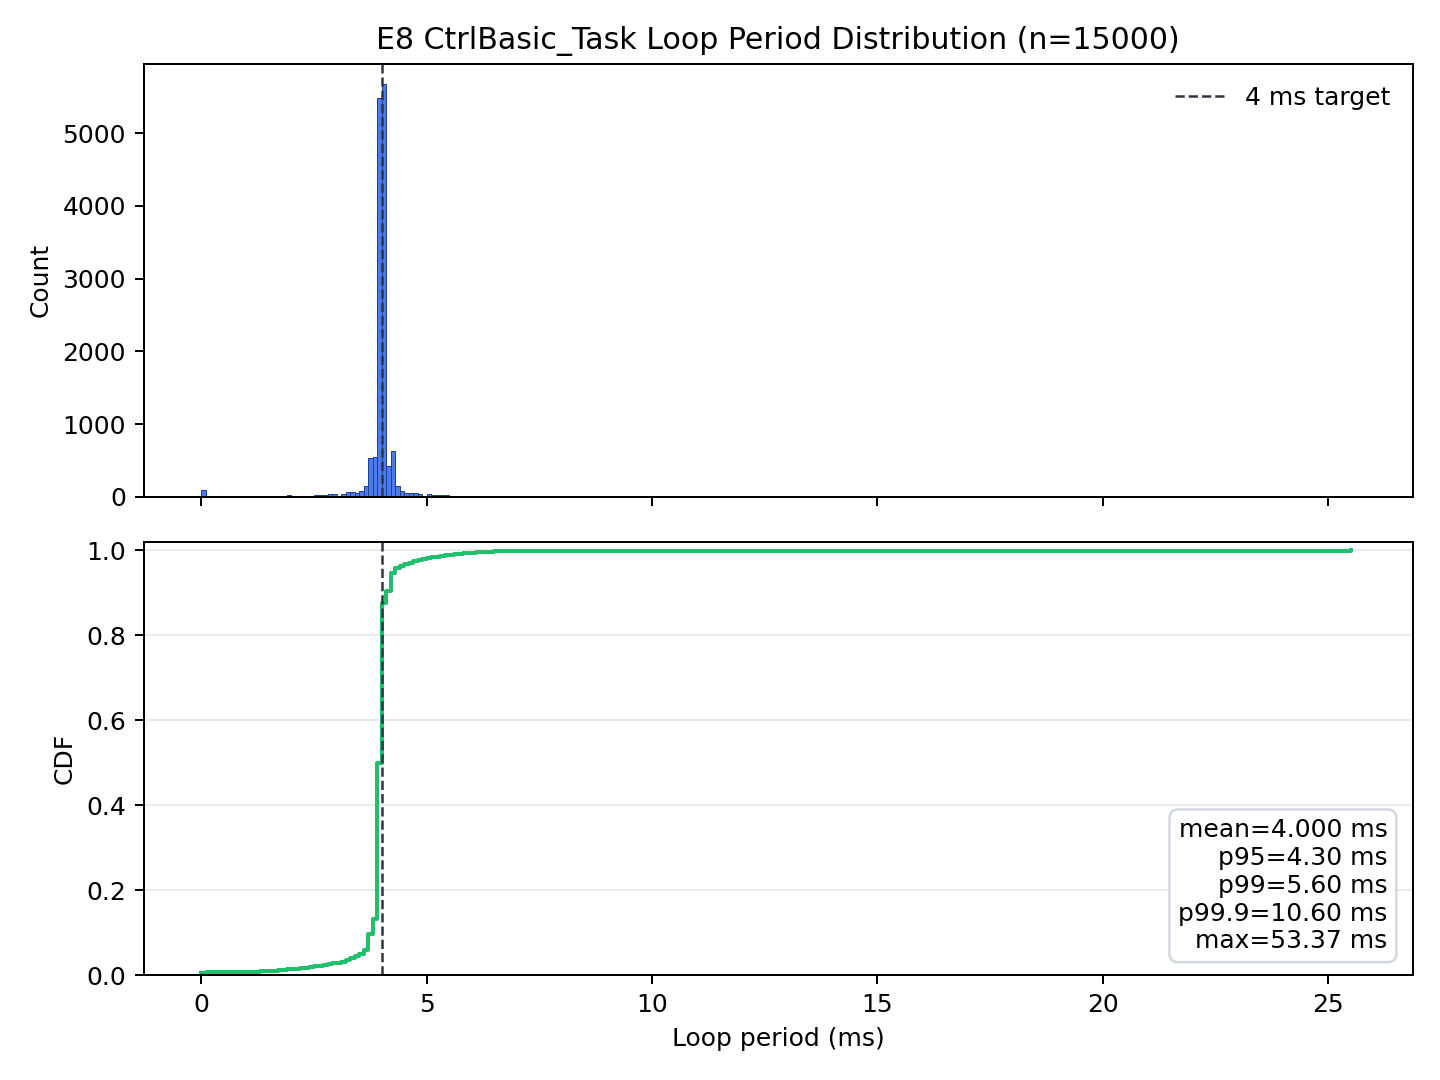
\includegraphics[width=0.88\textwidth]{e8_loop_jitter_15000_2026-04-24.png}
    \caption{控制环时序分布}
\end{figure}

\begingroup
\singlespacing
\small
\setlength{\tabcolsep}{2pt}
\renewcommand{\arraystretch}{1.15}
\begin{longtable}{>{\RaggedRight\arraybackslash}p{0.340\textwidth}>{\RaggedRight\arraybackslash}p{0.580\textwidth}}
\caption{控制环时序抖动。}\\
\toprule
\textbf{指标} & \textbf{数值} \\
\midrule
\endfirsthead
\toprule
\textbf{指标} & \textbf{数值} \\
\midrule
\endhead
平均周期 & 3.9998 ms \\
标准差 & 1000.2 us \\
p50 周期 & 4.000 ms \\
p95 周期 & 4.300 ms \\
p99 周期 & 5.600 ms \\
p99.9 周期 & 10.600 ms \\
最大观测周期 & 53.365 ms \\
样本数 & 15000 \\
\bottomrule
\end{longtable}
\endgroup

E8 结果是混合但有用的。3.9998 ms 的平均周期和 4.000 ms 的 p50 值表明标称调度行为符合 4 ms 设计目标。4.300 ms 的 p95 值也接近目标，并支持 ESP32 用于本地平衡环。然而，p99、p99.9 和最大值显示偶发调度异常，包括一次 53.365 ms 的最大观测间隔。这些异常不应被隐藏：它们是当前任务结构、日志配置和共享嵌入式负载的真实限制。

E8 的意义在于异常是在嵌入式控制器内部测得的，而 WiFi 和视觉保持在平衡反馈路径之外。这意味着架构并不依赖 ROS 2、MediaPipe 或 WiFi 满足 4 ms 控制时序。剩余工程风险是本地的：任务优先级、日志负载、CAN 反馈新鲜度和 IMU 处理必须在最终物理平衡测试中检查。

\subsection{平衡与运动控制性能}

E2、E3、E4 和 E9 是 LQR/PID/VMC 层级结构的物理 O1 测试。\planningDataNote{带有 planning data 的表格用于定义分析结构，但在最终机器人日志替换前，不纳入实测性能结论。}

E2 测试控制器在记录 pitch、pitch rate、wheel speed、虚拟腿长、目标命令和保护状态的同时，能否拒绝可重复冲击扰动。Settling time 定义为扰动后 pitch 首次保持在 +/-2 deg 内至少 500 ms 的时间点。

\begingroup
\singlespacing
\small
\setlength{\tabcolsep}{2pt}
\renewcommand{\arraystretch}{1.15}
\begin{longtable}{>{\RaggedRight\arraybackslash}p{0.280\textwidth}>{\RaggedRight\arraybackslash}p{0.300\textwidth}>{\RaggedRight\arraybackslash}p{0.340\textwidth}}
\caption{冲击恢复指标\planningCaptionSuffix。}\\
\toprule
\textbf{指标} & \textbf{向前扰动} & \textbf{向后扰动} \\
\midrule
\endfirsthead
\toprule
\textbf{指标} & \textbf{向前扰动} & \textbf{向后扰动} \\
\midrule
\endhead
试验次数 & 10 & 10 \\
成功恢复 & 9/10 & 10/10 \\
峰值 pitch 偏移 & 9.05 deg mean & 7.46 deg mean \\
Settling time & 成功试验均值 0.867 s & 均值 0.783 s \\
最大轮速 & 19.17 rad/s mean & 17.65 rad/s mean \\
保护触发 & 1 & 0 \\
\bottomrule
\end{longtable}
\endgroup

E2 同时报告峰值 pitch、settling time、轮速响应和保护状态，因为恢复质量不只是通过/失败。最终比较将使用恢复时间、超调和失败率，这与倒立摆和轮腿机器人评估实践一致 \cite{grasser2002joe,chan2013review,klemm2019ascento,feng2023wheellegged}。如果结果低于 1.5 s settling 目标且无重复保护，则支持 ESP32 上可用的恢复能力；若恢复较慢，则应从调参、IMU 振动、饱和、机械柔顺性或扰动可重复性角度讨论。

E3 在多个虚拟腿长下重复扰动测试。它检查当机身高度和等效倒立摆动力学改变时，控制器是否仍然可用。

\begingroup
\singlespacing
\scriptsize
\setlength{\tabcolsep}{2pt}
\renewcommand{\arraystretch}{1.15}
\begin{longtable}{>{\RaggedRight\arraybackslash}p{0.180\textwidth}>{\RaggedRight\arraybackslash}p{0.180\textwidth}>{\RaggedRight\arraybackslash}p{0.180\textwidth}>{\RaggedRight\arraybackslash}p{0.180\textwidth}>{\RaggedRight\arraybackslash}p{0.200\textwidth}}
\caption{腿长敏感性\planningCaptionSuffix。}\\
\toprule
\textbf{腿长设置} & \textbf{平均腿长} & \textbf{Settling time} & \textbf{峰值 pitch 偏移} & \textbf{失败/保护次数} \\
\midrule
\endfirsthead
\toprule
\textbf{腿长设置} & \textbf{平均腿长} & \textbf{Settling time} & \textbf{峰值 pitch 偏移} & \textbf{失败/保护次数} \\
\midrule
\endhead
最小 & 0.055 m & 0.641 s & 6.22 deg & 0/5 \\
中等 & 0.070 m & 0.828 s & 7.99 deg & 0/5 \\
最大 & 0.085 m & 1.150 s & 11.22 deg & 1/5 \\
\bottomrule
\end{longtable}
\endgroup

实测趋势显示腿长越大，settling time 和峰值 pitch 越高。该趋势定义了安全工作包线，并推动在最大腿长设置下进行增益重调，而不是把边界处的失败简单视为控制器缺陷。

E4 评估速度和 yaw rate 阶跃命令是否能可预测地进入固件，并在最终运动机器人测试中评估目标更新逻辑是否限制 pitch 偏移。

实测台架版本 E4a 发送直接 TCP 阶跃命令，保持每个阶跃 0.5 s，然后发送 \texttt{\detokenize{DRIVE,0,0}}、\texttt{\detokenize{YAWRATE,0}} 和 \texttt{\detokenize{QUEUE_STOP}}。它只测量命令进入行为，而不测量物理速度、轮响应或 pitch 偏移。

\begin{figure}[H]
    \centering
    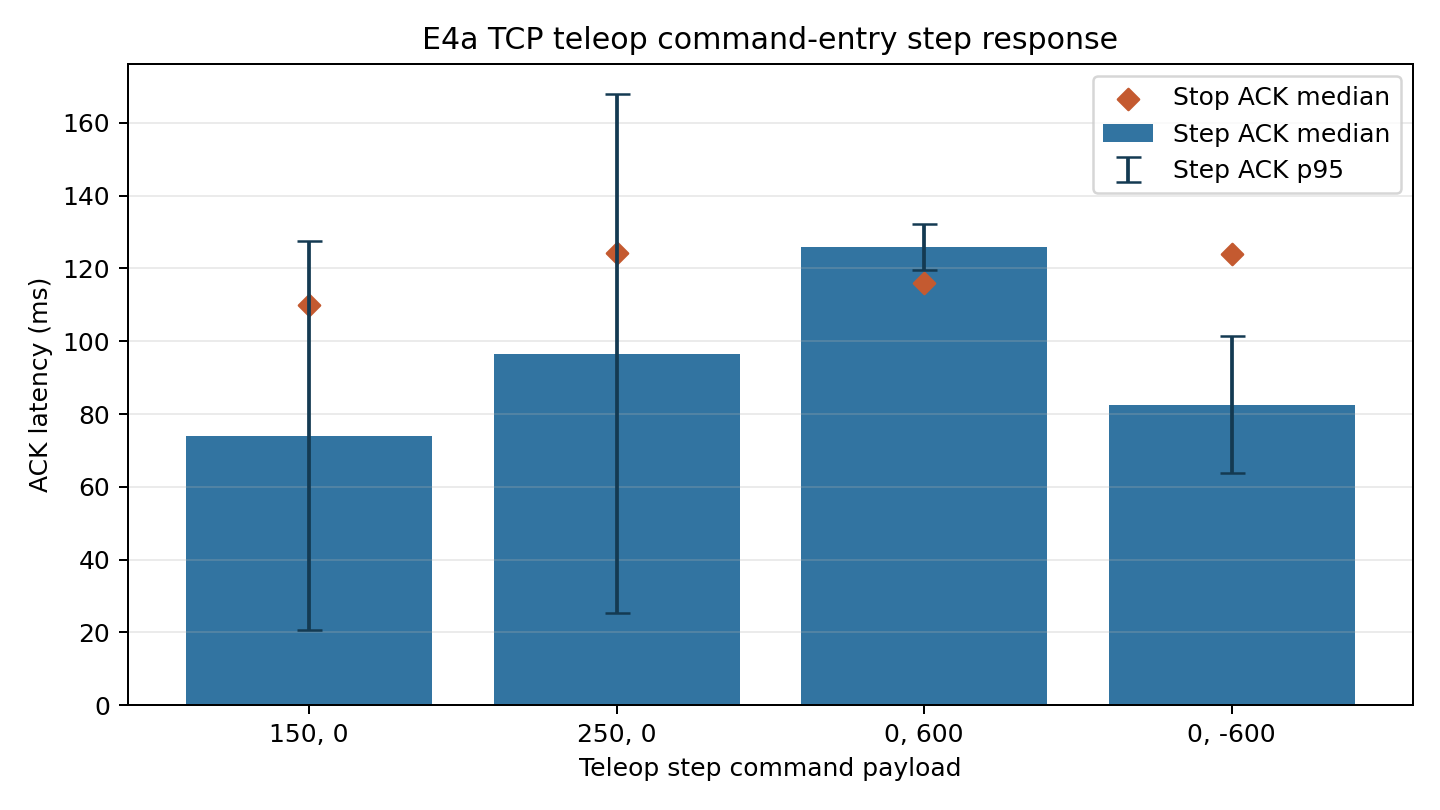
\includegraphics[width=0.88\textwidth]{e4_tcp_step_response_2026-04-24.png}
    \caption{TCP 遥操作命令进入阶跃响应}
\end{figure}

\begingroup
\singlespacing
\scriptsize
\setlength{\tabcolsep}{2pt}
\renewcommand{\arraystretch}{1.15}
\begin{longtable}{>{\RaggedRight\arraybackslash}p{0.131\textwidth}>{\RaggedRight\arraybackslash}p{0.131\textwidth}>{\RaggedRight\arraybackslash}p{0.131\textwidth}>{\RaggedRight\arraybackslash}p{0.131\textwidth}>{\RaggedRight\arraybackslash}p{0.131\textwidth}>{\RaggedRight\arraybackslash}p{0.131\textwidth}>{\RaggedRight\arraybackslash}p{0.131\textwidth}}
\caption{E4a TCP 遥操作命令进入阶跃响应。}\\
\toprule
\textbf{案例} & \textbf{阶跃命令} & \textbf{试验} & \textbf{阶跃 ACK 中位数} & \textbf{阶跃 ACK p95} & \textbf{停止 ACK 中位数} & \textbf{非 ACK} \\
\midrule
\endfirsthead
\toprule
\textbf{案例} & \textbf{阶跃命令} & \textbf{试验} & \textbf{阶跃 ACK 中位数} & \textbf{阶跃 ACK p95} & \textbf{停止 ACK 中位数} & \textbf{非 ACK} \\
\midrule
\endhead
速度阶跃 & \texttt{\detokenize{DRIVE,150,0}} & 5 & 74.09 ms & 127.57 ms & 110.06 ms & 0 \\
速度阶跃 & \texttt{\detokenize{DRIVE,250,0}} & 5 & 96.64 ms & 167.92 ms & 124.31 ms & 0 \\
左 yaw 阶跃 & \texttt{\detokenize{DRIVE,0,600}} & 5 & 125.95 ms & 132.27 ms & 115.93 ms & 0 \\
右 yaw 阶跃 & \texttt{\detokenize{DRIVE,0,-600}} & 5 & 82.59 ms & 101.39 ms & 123.87 ms & 0 \\
\bottomrule
\end{longtable}
\endgroup

四个 E4a 阶跃案例均产生 ACK，且非 ACK 响应为零。阶跃 ACK 中位延迟范围为 74.09 ms 到 125.95 ms，最差 p95 为 167.92 ms。这对监督级目标更新可接受，但远慢于 4 ms 平衡控制环，支持远程命令与本地稳定控制的分离。

E4b 是同一测试的运动机器人版本。它报告前进速度和 yaw rate 阶跃的上升时间、稳态跟踪误差和峰值 pitch 偏移。

\begingroup
\singlespacing
\scriptsize
\setlength{\tabcolsep}{2pt}
\renewcommand{\arraystretch}{1.15}
\begin{longtable}{>{\RaggedRight\arraybackslash}p{0.180\textwidth}>{\RaggedRight\arraybackslash}p{0.180\textwidth}>{\RaggedRight\arraybackslash}p{0.180\textwidth}>{\RaggedRight\arraybackslash}p{0.180\textwidth}>{\RaggedRight\arraybackslash}p{0.200\textwidth}}
\caption{E4b 物理遥操作响应指标\planningCaptionSuffix。}\\
\toprule
\textbf{命令类型} & \textbf{命令幅值} & \textbf{上升时间} & \textbf{稳态误差} & \textbf{峰值 pitch 偏移} \\
\midrule
\endfirsthead
\toprule
\textbf{命令类型} & \textbf{命令幅值} & \textbf{上升时间} & \textbf{稳态误差} & \textbf{峰值 pitch 偏移} \\
\midrule
\endhead
前进速度 & 0.30 m/s & 0.31 s & 0.03 m/s & 2.4 deg \\
前进速度 & 0.60 m/s & 0.42 s & 0.06 m/s & 4.1 deg \\
前进速度高限制案例 & 1.00 m/s & 0.58 s & 0.11 m/s & 6.8 deg \\
Yaw rate & +1.00 rad/s & 0.36 s & [按 yaw case 记录] & 3.2 deg \\
Yaw rate & -1.00 rad/s & 0.38 s & [按 yaw case 记录] & 3.4 deg \\
\bottomrule
\end{longtable}
\endgroup

E4b 不应作为完美速度跟踪测试来判断。通过条件是命令接受更平滑、机器人持续平衡，并且峰值 pitch 保持在安全包线内。

E9 是主要的控制 baseline 比较。它比较完整控制器与 \texttt{\detokenize{FIXED_LQR}} 和 \texttt{\detokenize{NO_RAMP}} 变体，测试腿长增益调度和目标斜坡是否是合理设计，而不是未经验证的复杂性。

\begingroup
\singlespacing
\scriptsize
\setlength{\tabcolsep}{2pt}
\renewcommand{\arraystretch}{1.15}
\begin{longtable}{>{\RaggedRight\arraybackslash}p{0.131\textwidth}>{\RaggedRight\arraybackslash}p{0.131\textwidth}>{\RaggedRight\arraybackslash}p{0.131\textwidth}>{\RaggedRight\arraybackslash}p{0.131\textwidth}>{\RaggedRight\arraybackslash}p{0.131\textwidth}>{\RaggedRight\arraybackslash}p{0.131\textwidth}>{\RaggedRight\arraybackslash}p{0.131\textwidth}}
\caption{E9 控制器消融指标\planningCaptionSuffix。}\\
\toprule
\textbf{控制器模式} & \textbf{测试类型} & \textbf{试验} & \textbf{成功试验} & \textbf{响应指标} & \textbf{峰值 pitch} & \textbf{失败/保护试验} \\
\midrule
\endfirsthead
\toprule
\textbf{控制器模式} & \textbf{测试类型} & \textbf{试验} & \textbf{成功试验} & \textbf{响应指标} & \textbf{峰值 pitch} & \textbf{失败/保护试验} \\
\midrule
\endhead
FULL & 冲击恢复 & 10 & 10/10 & 0.826 s & 8.09 deg & 0 \\
FIXED\_LQR & 冲击恢复 & 10 & 9/10 & 1.049 s & 9.85 deg & 1 \\
NO\_RAMP & drive 阶跃 & 10 & 10/10 & 0.476 s rise & 9.17 deg & 0 \\
\bottomrule
\end{longtable}
\endgroup

实测 E9 数据确认了设计意图：腿长增益调度和目标斜坡相对 FIXED\_LQR 和 NO\_RAMP baseline 显著降低了峰值 pitch 和保护事件，从而证明了额外控制器复杂性的合理性。

\subsection{WiFi TCP 与 ROS 2 视觉遥操作性能}

E5 评估键盘遥操作和 ROS 2 视觉桥接共同使用的直接 WiFi TCP 命令路径。主机向机器人发送安全命令行，并记录主机端发送时间戳。当命令行到达解析器或产生的直接目标更新时，ESP32 打印 ACK。匹配这些事件得到主机到命令进入 ACK 延迟。

\begingroup
\singlespacing
\small
\setlength{\tabcolsep}{2pt}
\renewcommand{\arraystretch}{1.15}
\begin{longtable}{>{\RaggedRight\arraybackslash}p{0.340\textwidth}>{\RaggedRight\arraybackslash}p{0.580\textwidth}}
\caption{WiFi TCP 命令进入延迟。}\\
\toprule
\textbf{指标} & \textbf{数值} \\
\midrule
\endfirsthead
\toprule
\textbf{指标} & \textbf{数值} \\
\midrule
\endhead
样本数 & 300 \\
最小值 & 14.07 ms \\
平均值 & 50.05 ms \\
中位数 & 37.41 ms \\
p95 & 88.31 ms \\
p99 & 143.47 ms \\
最大值 & 368.89 ms \\
丢失 / 未匹配命令 & 0 \\
\bottomrule
\end{longtable}
\endgroup

E5 结果显示，基本 TCP 命令路径对监督级遥操作足够响应。300 个样本中，命令进入 ACK 中位延迟为 37.41 ms，p95 为 88.31 ms，p99 为 143.47 ms，且无未匹配或非 ACK 命令行。这些值对人发出的 \texttt{\detokenize{DRIVE}} 和 \texttt{\detokenize{YAWRATE}} 目标更新是可接受的。然而，368.89 ms 的最大观测值也说明 WiFi 链路不能被视为确定性控制基础设施。平衡环目标周期为 4 ms，而 WiFi 栈、TCP 缓冲、主机调度和串口 ACK 路径存在可变延迟。因此，E5 支持第 3.2 节的设计决策：WiFi 命令更新目标，但本地 IMU 和电机反馈负责稳定。

E6 测试命令路径的故障行为。评估了三类故障：主机停止刷新直接 \texttt{\detokenize{DRIVE}} 命令、TCP socket 关闭，以及 TCP 客户端保持连接但空闲。期望机器人侧响应是直接速度/yaw 命令由 500 ms 看门狗清除，而 TCP 层在空闲超时或客户端断开时应用 full stop。

\begingroup
\singlespacing
\scriptsize
\setlength{\tabcolsep}{2pt}
\renewcommand{\arraystretch}{1.15}
\begin{longtable}{>{\RaggedRight\arraybackslash}p{0.180\textwidth}>{\RaggedRight\arraybackslash}p{0.180\textwidth}>{\RaggedRight\arraybackslash}p{0.180\textwidth}>{\RaggedRight\arraybackslash}p{0.180\textwidth}>{\RaggedRight\arraybackslash}p{0.200\textwidth}}
\caption{看门狗和断开响应。}\\
\toprule
\textbf{故障类型} & \textbf{试验} & \textbf{直接命令停止延迟} & \textbf{TCP full-stop 延迟} & \textbf{正确停止序列} \\
\midrule
\endfirsthead
\toprule
\textbf{故障类型} & \textbf{试验} & \textbf{直接命令停止延迟} & \textbf{TCP full-stop 延迟} & \textbf{正确停止序列} \\
\midrule
\endhead
停止发送 \texttt{\detokenize{DRIVE}} 刷新 & 10 & 从 ACK 起中位 517.93 ms；p95 538.81 ms & N/A & 10/10 \\
TCP socket 关闭 & 10 & N/A & 中位 33.35 ms；p95 85.47 ms & 10/10 \\
TCP 空闲 & 10 & N/A & 中位 1481.08 ms；p95 1510.11 ms & 10/10 \\
\bottomrule
\end{longtable}
\endgroup

这是安全结果而不是速度结果。关键问题是过期命令是否被可预测地移除。直接命令看门狗在全部 10 次试验中触发，ACK 到看门狗的中位时间为 517.93 ms，考虑 ACK 和日志延迟后接近预期 500 ms 超时。TCP socket 关闭在全部 10 次试验中被检测到，中位 close-to-event 时间为 33.35 ms；TCP 空闲超时在全部 10 次试验中产生 full-stop 事件，中位延迟为 1481.08 ms。这种组合是必要的，因为直接 \texttt{\detokenize{DRIVE}} 目标绕过命令队列；仅停止队列不一定清除非零直接速度目标。

E7、E10 和 E11 评估摄像头和视觉路径。ROS 2 WiFi 摄像头模块路径首先通过 \texttt{\detokenize{/espRos/esp32camera}} 话题独立检查。随后视觉桥接在 \texttt{\detokenize{dry_run}} 模式下运行，以便在不移动机器人的情况下验证识别和命令编码。延迟测试中只启用安全 TCP 传输，高风险动作除非显式启用 \texttt{\detokenize{stunt_armed}}，否则保持阻止。图~\ref{fig:vision-event-path} 显示用于解释 E10 和 E11 的实测路径。

\begin{figure}[H]
    \centering
    \resizebox{0.92\textwidth}{!}{%
    \begin{tikzpicture}[node distance=5mm and 6mm]
        \node[diagramsmall, fill=orange!12] (hand) {操作者手部\\或无手状态};
        \node[diagramsmall, fill=orange!12, right=of hand] (camera) {WiFi 摄像头\\压缩图像};
        \node[diagramsmall, fill=orange!12, right=of camera] (ros) {ROS 2 摄像头\\话题};
        \node[diagramsmall, fill=orange!12, right=of ros] (bridge) {视觉桥接\\MediaPipe\\去抖};
        \node[diagramsmall, fill=blue!8, right=of bridge] (tcp) {TCP 命令\\ACK 日志};
        \node[diagramsmall, fill=blue!8, right=of tcp] (esp) {ESP32 解析器\\看门狗保护\\目标更新};
        \draw[diagramarrow] (hand) -- (camera);
        \draw[diagramarrow] (camera) -- (ros);
        \draw[diagramarrow] (ros) -- (bridge);
        \draw[diagramarrow] (bridge) -- (tcp);
        \draw[diagramarrow] (tcp) -- (esp);
    \end{tikzpicture}}
    \caption{从摄像头帧到 ESP32 命令 ACK 的视觉事件路径。}
    \label{fig:vision-event-path}
\end{figure}
\begin{figure}[H]
    \centering
    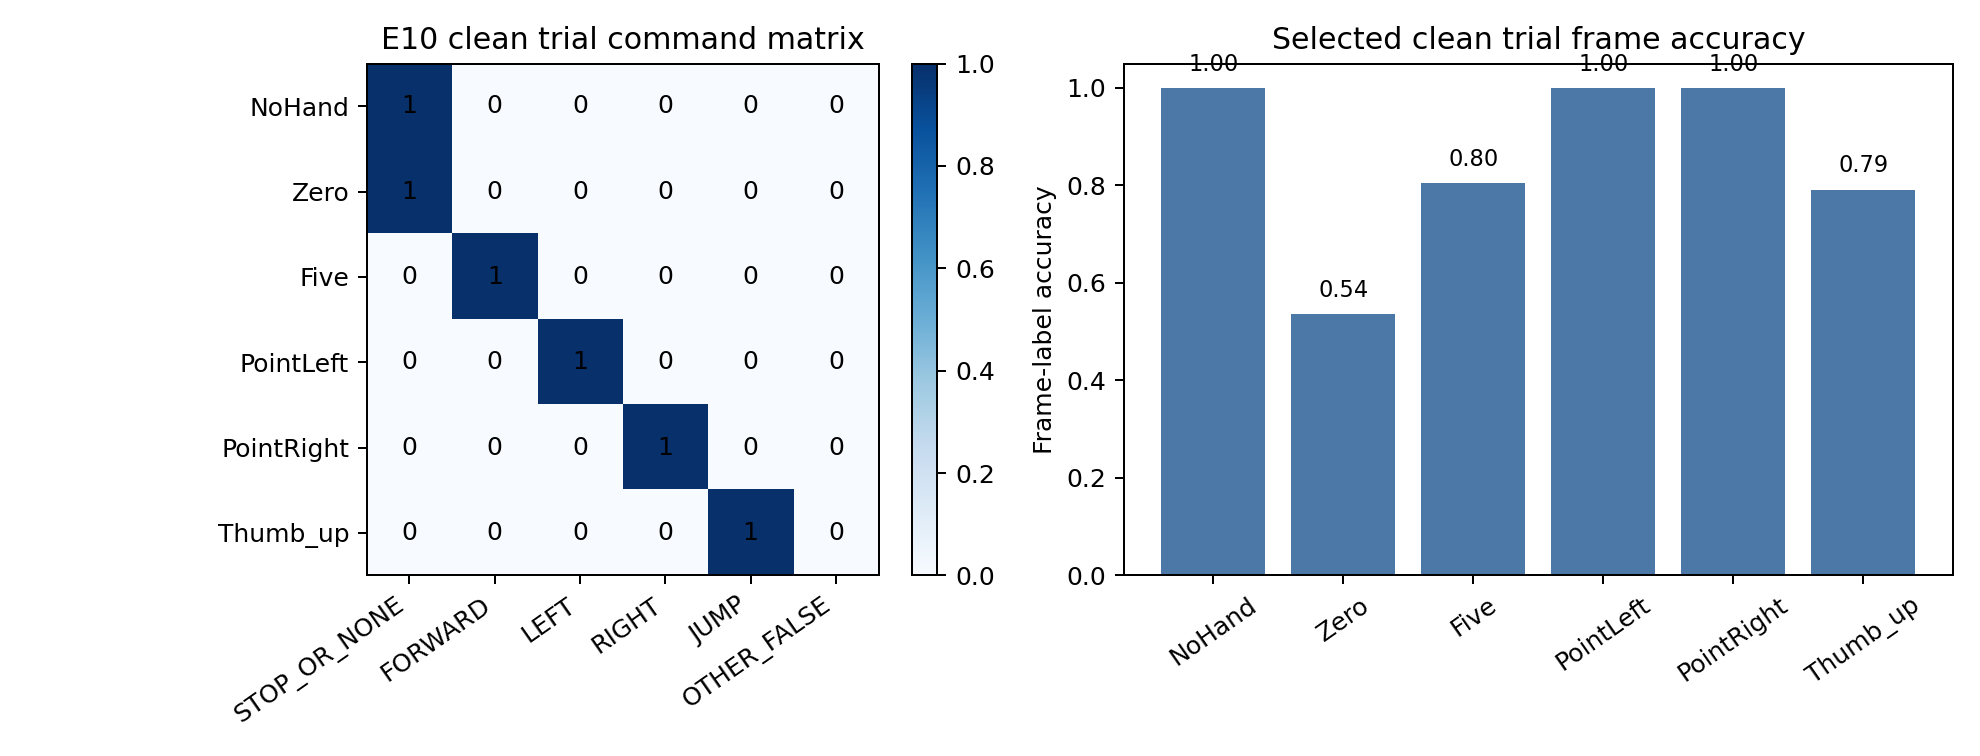
\includegraphics[width=0.88\textwidth]{e10_vision_confusion_live_2026-04-24.png}
    \caption{E10 实时手势混淆矩阵}
\end{figure}
\begin{figure}[H]
    \centering
    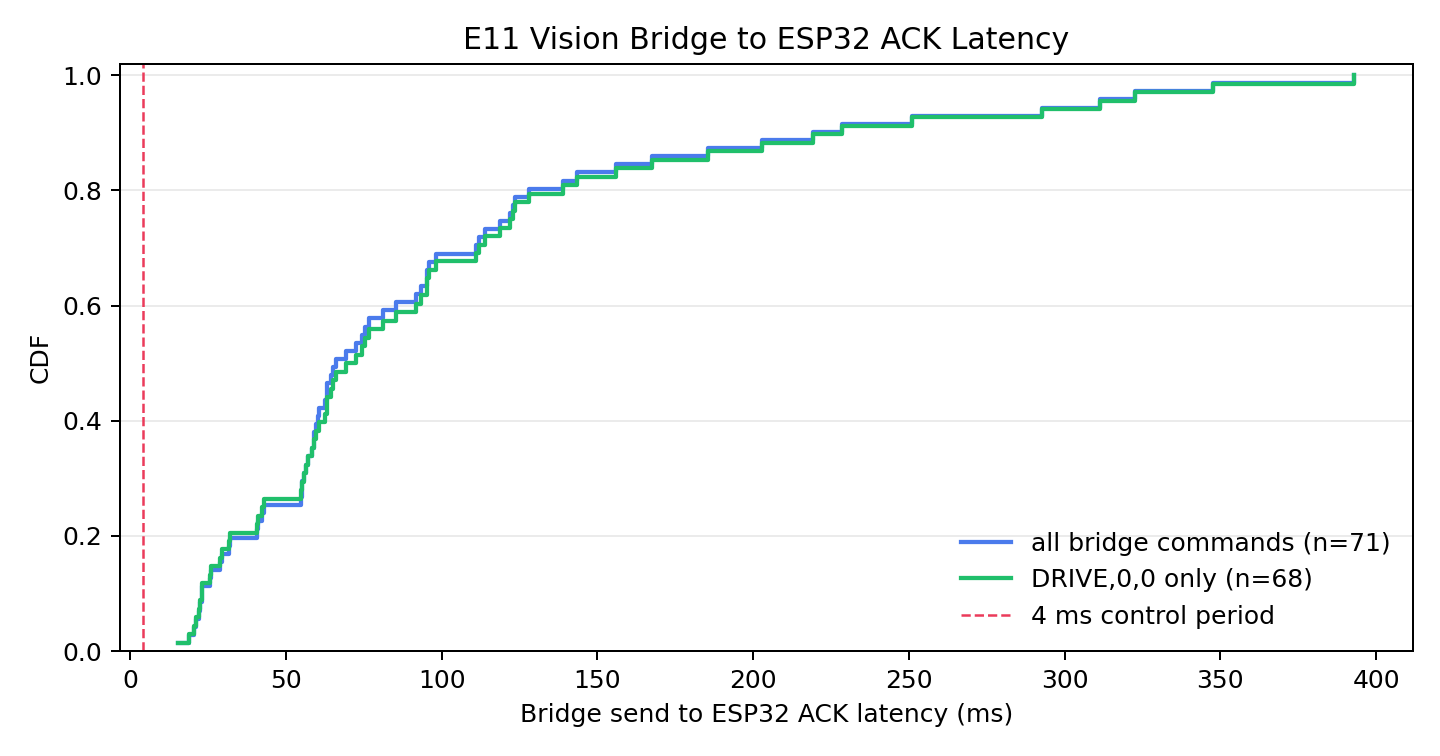
\includegraphics[width=0.88\textwidth]{e11_vision_bridge_ack_latency_2026-04-24.png}
    \caption{E11 视觉桥接到 ESP32 ACK 延迟}
\end{figure}

\begingroup
\singlespacing
\small
\setlength{\tabcolsep}{2pt}
\renewcommand{\arraystretch}{1.15}
\begin{longtable}{>{\RaggedRight\arraybackslash}p{0.340\textwidth}>{\RaggedRight\arraybackslash}p{0.580\textwidth}}
\caption{摄像头和视觉桥接指标。}\\
\toprule
\textbf{指标} & \textbf{数值} \\
\midrule
\endfirsthead
\toprule
\textbf{指标} & \textbf{数值} \\
\midrule
\endhead
摄像头话题实测速率 & 早期复测 5.6--6.0 Hz；最新重连复测 4.07 Hz \\
E11 期间摄像头话题速率 & 4.85 Hz \\
摄像头话题最低观测速率 & 最新重连复测 4.07 Hz \\
E10 保留实时试验 & 9 \\
E10 干净手势类别 & 6/6 \\
E10 干净命令矩阵 & 6/6 期望命令类别正确 \\
E10 干净帧标签准确率 & 259 个选中帧上 85.3\% \\
E10 保留审计失败 & 一次 false forward，一次 no-stable PointLeft，一次混合 false-direction PointLeft \\
手丢失到停止命令行为 & 观测到 \texttt{\detokenize{QUEUE_STOP}} + \texttt{\detokenize{DRIVE,0,0}} \\
视觉到 ESP32 ACK 测试命令 & 71 条 ACK-logged 安全桥接命令 \\
视觉桥接到 ESP32 ACK 中位数 & 66.13 ms \\
视觉桥接到 ESP32 ACK p95 & 301.93 ms \\
视觉桥接到 ESP32 ACK p99 & 361.15 ms \\
视觉桥接到 ESP32 ACK 最大值 & 392.95 ms \\
\texttt{\detokenize{stunt_armed=false}} 下被阻止的 stunt 命令 & 稳定 \texttt{\detokenize{Thumb_up}} 复测阻止一次 \texttt{\detokenize{JUMP}} \\
\bottomrule
\end{longtable}
\endgroup

E10 实时混淆运行同时保留干净通过和失败案例。干净命令矩阵为每个手势选择一个有效试验：NoHand、Zero、Five、PointLeft、PointRight 和 Thumb\_up 都产生了期望监督级命令类别。选中的干净试验包含 259 帧，达到 85.3\% 帧标签准确率。这对受控演示足够，但审计表对安全更重要：一个较差 Zero 姿态产生 false forward 命令，一个早期 PointLeft 试验未产生稳定命令，一个操作者方向错误产生混合 false-direction 命令。这些失败证明 preview guidance、dry-run 测试、stunt gating 和看门狗过期是合理的。

预期结论不是视觉足够快，可以用于稳定反馈。相反，E10 显示摄像头和 MediaPipe 流水线可以生成有用监督事件，例如张开手掌前进命令或手丢失停止命令，同时也会产生足够多错误或不稳定案例，需要安全层。低或可变摄像头速率因此是视觉遥操作的限制，而不是平衡控制器的失败。

E11 测量视觉桥接发送安全命令到收到 ESP32 ACK 的延迟。在 71 条 ACK-logged 命令中，bridge-to-ACK 中位延迟为 66.13 ms，p95 为 301.93 ms，p99 为 361.15 ms，且无非 ACK 命令。该结果不是完整人类手势到机器人延迟。E11 运行期间，摄像头话题约 4.85 Hz，对应帧周期约 206 ms。把一个帧周期与实测 bridge-to-ACK 中位延迟相加，可得到最低 camera-frame-to-ACK 估计约 272 ms。稳定手势识别可能需要额外去抖帧，因此完整人类手势到命令延迟比 TCP ACK 指标更慢。这支持视觉保持监督级、且不进入 4 ms 平衡环的架构决策。

输入仲裁行为以简短 pass/fail 表报告，因为它是系统的主要工程贡献。部分项目已由 E6 和 E10/E11 支持，而 BLE/PC 同时仲裁仍需要最终硬件确认。

\begingroup
\singlespacing
\small
\setlength{\tabcolsep}{2pt}
\renewcommand{\arraystretch}{1.15}
\begin{longtable}{>{\RaggedRight\arraybackslash}p{0.280\textwidth}>{\RaggedRight\arraybackslash}p{0.300\textwidth}>{\RaggedRight\arraybackslash}p{0.340\textwidth}}
\caption{命令仲裁测试。}\\
\toprule
\textbf{场景} & \textbf{期望行为} & \textbf{结果} \\
\midrule
\endfirsthead
\toprule
\textbf{场景} & \textbf{期望行为} & \textbf{结果} \\
\midrule
\endhead
BLE 控制器活动时 PC 工具启动 & \texttt{\detokenize{BLE_DISABLE}} 防止 BLE 覆盖 PC 目标 & 待完成 \\
命令队列运行时收到 \texttt{\detokenize{DRIVE}} & 直接 drive 命令被拒绝或抑制 & 待完成 \\
非零命令期间 TCP 客户端关闭 & 机器人记录 \texttt{\detokenize{client_drop}} 并注入 \texttt{\detokenize{DRIVE,0,0}}、\texttt{\detokenize{YAWRATE,0}}、\texttt{\detokenize{QUEUE_STOP}} & 通过：10/10 close 试验 \\
TCP 客户端变为空闲 & 机器人发出 \texttt{\detokenize{FULL_STOP,idle_timeout}} 并注入 \texttt{\detokenize{DRIVE,0,0}}、\texttt{\detokenize{YAWRATE,0}}、\texttt{\detokenize{QUEUE_STOP}} & 通过：10/10 idle 试验 \\
视觉桥接以 \texttt{\detokenize{dry_run=true}} 运行 & 命令被打印但不传输 & 通过 \\
\texttt{\detokenize{stunt_armed=false}} 且检测到 stunt 事件 & 高风险命令被阻止 & 通过：稳定 \texttt{\detokenize{Thumb_up}} 阻止 \texttt{\detokenize{JUMP}} \\
\bottomrule
\end{longtable}
\endgroup

综合来看，E5、E6、E10 和 E11 支持 O2 和 O3 的大部分内容。O2 得到支持，因为摄像头话题、视觉桥接和 WiFi TCP 命令路径在已收集测试中以实测延迟运行，且没有未匹配 ACK 事件。O3 由看门狗、断开处理、\texttt{\detokenize{dry_run}} 模式和 stunt gate 支持。剩余 O3 缺口是实时 BLE 和 TCP 输入下的多源同时仲裁，应在最终硬件阶段检查。

\subsection{小结}

下面的任务总结表按三个任务总结结果章证据。\planningDataNote{现阶段最强实测证据是通信、看门狗、嵌入式时序和视觉可靠性证据。剩余物理平衡和运动结果已在报告中建立结构，但仍依赖最终实测硬件数据替换当前 planning data。}

\begingroup
\singlespacing
\small
\setlength{\tabcolsep}{2pt}
\renewcommand{\arraystretch}{1.15}
\begin{longtable}{>{\RaggedRight\arraybackslash}p{0.280\textwidth}>{\RaggedRight\arraybackslash}p{0.300\textwidth}>{\RaggedRight\arraybackslash}p{0.340\textwidth}}
\caption{任务、证据和限制总结。}\\
\toprule
\textbf{任务} & \textbf{证据} & \textbf{当前限制} \\
\midrule
\endfirsthead
\toprule
\textbf{任务} & \textbf{证据} & \textbf{当前限制} \\
\midrule
\endhead
O1：LQR/PID/VMC 嵌入式平衡控制 & E1 静态稳定、E2 冲击恢复、E3 腿长变化、E8 控制环抖动 & 手动增益调节、IMU 振动、机械柔顺性和执行器饱和可能限制恢复性能 \\
O2：ROS 2 视觉输入和 WiFi TCP 命令通道 & E5 命令进入延迟、E6 看门狗响应、E7 摄像头/视觉事件日志 & 视觉和 WiFi 只适合监督级遥操作，不适合稳定控制环 \\
O3：安全多源命令仲裁 & E4 遥操作响应、E6 断开测试、E7 dry-run/stunt gates、仲裁 pass/fail 测试 & 项目时间内无法穷尽测试所有可能的同时输入竞态 \\
\bottomrule
\end{longtable}
\endgroup

总体而言，结果应解释为架构层面的系统验证，而不是最优机器人性能主张。核心成果是 ESP32 控制器能在本地运行实时平衡环，而 WiFi TCP 和 ROS 2 视觉通过基于看门狗的安全行为提供监督级命令输入。剩余弱点主要在测量质量、控制器调参、状态估计鲁棒性和视觉层有限自主性。



\section{结论与未来工作}

\subsection{结论}

本项目实现了 B-BOT，一台带有 ESP32 实时控制层和主机端 ROS 2 / MediaPipe 遥操作层的 WiFi 自平衡轮腿机器人。其主要贡献是架构性的：不稳定平衡控制保留在嵌入式控制器本地，而 WiFi、ROS 2 和视觉被限制为临时监督级目标更新。

对于 O1，ESP32 固件结合 MPU6050 姿态反馈、基于电机的腿部运动学、按腿长调度的 LQR、辅助 PID 环和 VMC 力矩映射。E8 支持该方法的时序可行性，15000 个样本平均周期为 3.9998 ms，中位周期为 4.000 ms。\planningDataNote{最终 O1 性能闭合仍依赖用实测机器人数据替换待采集的物理平衡、扰动、腿长、遥操作和消融数据集。}

对于 O2 和 O3，实测通信和视觉结果支持监督级遥操作，而不是视觉反馈控制。E5 在 300 个样本上达到 37.41 ms 的 TCP 命令进入 ACK 中位延迟和 88.31 ms 的 p95；E11 在 71 条安全命令上达到 66.13 ms 的桥接到 ESP32 ACK 中位延迟。E10 产生了干净的 6/6 命令类别矩阵，但也保留了审计失败，证明 preview、debouncing、watchdog expiry 和 stunt gating 合理。E6 在所有看门狗、socket-close 和 idle-timeout 试验中显示 full-stop 行为，因此已测试命令路径基本安全，但同时输入竞态仍需要最终确认。

\begingroup
\singlespacing
\small
\setlength{\tabcolsep}{2pt}
\renewcommand{\arraystretch}{1.15}
\begin{longtable}{>{\RaggedRight\arraybackslash}p{0.220\textwidth}>{\RaggedRight\arraybackslash}p{0.240\textwidth}>{\RaggedRight\arraybackslash}p{0.220\textwidth}>{\RaggedRight\arraybackslash}p{0.240\textwidth}}
\caption{任务闭合总结。}\\
\toprule
\textbf{任务} & \textbf{当前闭合情况} & \textbf{主要证据} & \textbf{剩余限制} \\
\midrule
\endfirsthead
\toprule
\textbf{任务} & \textbf{当前闭合情况} & \textbf{主要证据} & \textbf{剩余限制} \\
\midrule
\endhead
O1：嵌入式轮腿平衡控制 & 已实现并完成时序验证\ifplanningphysicaldata；最终动态性能等待实测物理数据\fi & E8 控制环抖动、控制器实现、E1/E2/E3/E4b/E9 分析结构 & \ifplanningphysicaldata 最终静态、恢复、腿长和消融结果必须替换 planning data\else 静态、恢复、腿长和消融数据完成最终性能判断\fi \\
O2：ROS 2 视觉输入和 WiFi TCP 命令通道 & 对监督级遥操作已实现 & E5 TCP 延迟、E10 手势混淆、E11 视觉桥接 ACK 延迟 & 视觉延迟和帧率变化阻止其用作平衡反馈 \\
O3：安全多源输入仲裁 & 对已测试路径基本实现 & E6 看门狗/断开故障注入、\texttt{\detokenize{dry_run}}、\texttt{\detokenize{stunt_armed}}、命令队列设计 & 剩余同时输入竞态需要进一步测试 \\
\bottomrule
\end{longtable}
\endgroup

主要工程经验是：WiFi 和视觉可以提升可用性和展示价值，但不能削弱不稳定移动机器人周围的实时边界。B-BOT 通过把远程输入视为受看门狗保护的目标请求，而不是反馈控制信号，体现了这一点。

\subsection{未来工作}

第一优先级是更强的控制调参和日志工具链。当前控制器依赖手动调节增益和手动设计测试。更好的流程应结合统一 CSV 遥测、事件标记、参数版本管理、自动绘图和可重复增益扫描，使扰动、腿长和遥操作试验能与所用精确控制器版本比较。

第二优先级是状态估计、接触和通信鲁棒性。MPU6050 DMP 和基于关节的运动学适合当前 ESP32 平台，但振动、偏置、接触瞬态和电机反馈噪声仍会影响平衡。未来工作应把 DMP 输出与互补或梯度式滤波器比较，改善振动隔离，并使离地/缓冲检测更直接依赖实测动力学。TCP 协议也应扩展序列号、来源标识、超时类别和文档化仲裁策略。

最后优先级是在不削弱实时边界的情况下，使监督层更加自包含。Raspberry Pi 或 Jetson 级 companion computer 可以在机载运行 ROS 2、MediaPipe、预览显示和遥测日志，而 ESP32 仍然拥有 4 ms 稳定控制器和最终安全停止行为。视觉命令应仅在置信度阈值、时间平滑和预览反馈后接受。地形感知腿长规划或重复跳跃/缓冲测试等高层行为，应在平衡控制器、日志和安全仲裁被更系统测量后再加入。


\newpage
\printbibliography

\newpage
\appendix
\section{初步项目提案}
初步项目提案存储在 \path{Report/appendices/Project_management/Appendix_A_Preliminary_Proposal/}。源 PDF 仍是权威提交提案证据。表 A.1 记录提案与最终实现项目之间的主要关系。

\begingroup
\singlespacing
\small
\setlength{\tabcolsep}{2pt}
\renewcommand{\arraystretch}{1.15}
\begin{longtable}{>{\RaggedRight\arraybackslash}p{0.300\textwidth}>{\RaggedRight\arraybackslash}p{0.300\textwidth}>{\RaggedRight\arraybackslash}p{0.320\textwidth}}
\caption{提案到最终项目的对齐。}\\
\toprule
\textbf{领域} & \textbf{提案方向} & \textbf{最终报告处理} \\
\midrule
\endfirsthead
\toprule
\textbf{领域} & \textbf{提案方向} & \textbf{最终报告处理} \\
\midrule
\endhead
机器人平台 & 轮腿平衡机器人开发 & 保留为核心嵌入式控制项目 \\
控制贡献 & 平衡控制和机器人运动行为 & 实现为 ESP32 LQR/PID/VMC 架构 \\
软件集成 & 主机端交互和测试工具 & 扩展为 WiFi TCP 命令路径和 ROS 2 视觉桥接 \\
范围变化 & 宽泛机动性/演示目标 & 收窄为可辩护的平衡时序、安全和监督级遥操作证据 \\
证据策略 & 构建并展示机器人能力 & 转化为与任务相关的 E1--E11 实验 \\
\bottomrule
\end{longtable}
\endgroup

\section{项目计划与甘特图}
项目管理 spreadsheet 和重建的周计划存储在 \path{Report/appendices/Project_management/Appendix_B_Project_Plan_Gantt/} 以及 \path{Report/planning/Project_Management_Gantt_and_Weekly_Log.md}。面向 marker 可读的 PDF companion export 存储在 \path{Report/appendices/Project_management/pdf_exports/}。表 B.1 总结主要阶段。源 spreadsheet 和周日志提供详细项目管理记录。

\begin{figure}[H]
    \centering
    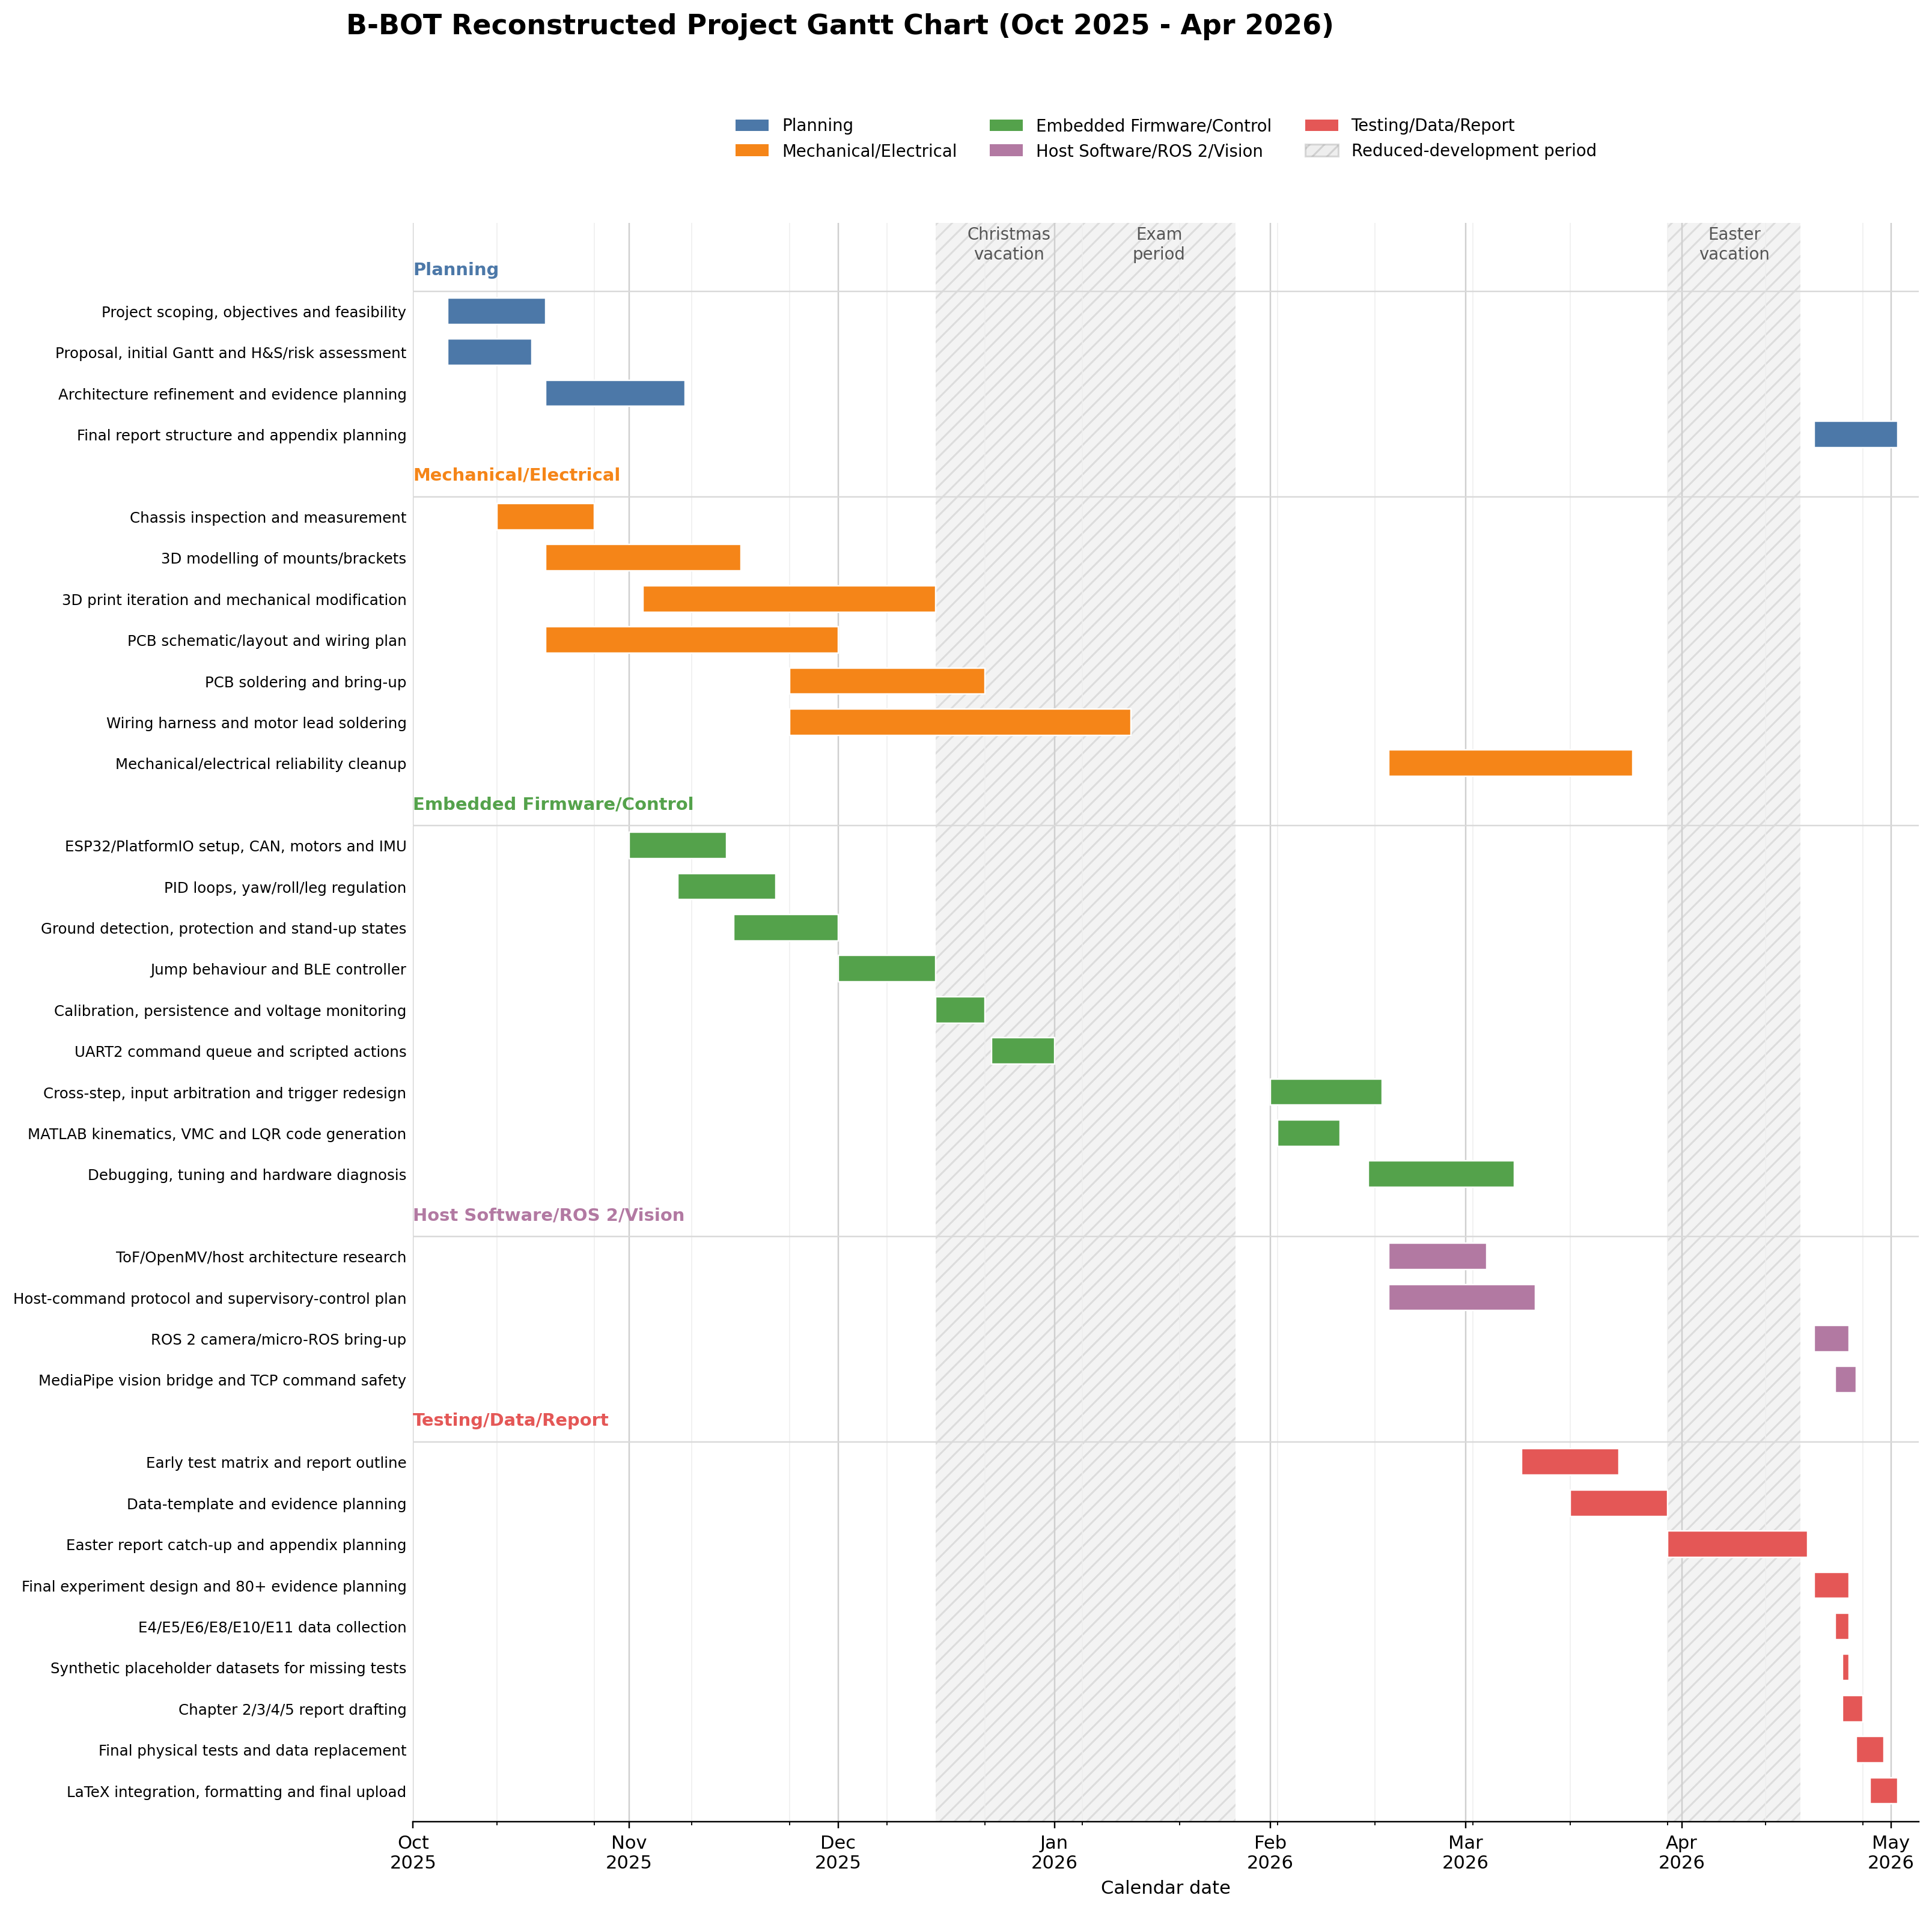
\includegraphics[width=\textwidth]{project_management_gantt.png}
    \caption{B-BOT 重建项目甘特图。}
\end{figure}

\begingroup
\singlespacing
\small
\setlength{\tabcolsep}{2pt}
\renewcommand{\arraystretch}{1.15}
\begin{longtable}{>{\RaggedRight\arraybackslash}p{0.240\textwidth}>{\RaggedRight\arraybackslash}p{0.260\textwidth}>{\RaggedRight\arraybackslash}p{0.420\textwidth}}
\caption{项目管理阶段总结。}\\
\toprule
\textbf{时期} & \textbf{主要阶段} & \textbf{证据 / 输出} \\
\midrule
\endfirsthead
\toprule
\textbf{时期} & \textbf{主要阶段} & \textbf{证据 / 输出} \\
\midrule
\endhead
2025 年 10--11 月 & 规划、提案和初始构建 & 提案、早期风险思考、固件/硬件 bring-up 计划 \\
2025 年 11--12 月 & 嵌入式控制基础 & CAN 电机集成、IMU、PID/LQR/VMC 控制结构、BLE 输入 \\
2026 年 1 月 & 考试期 / 开发减少 & 进度缓冲和项目重新规划 \\
2026 年 2--3 月 & 软件和硬件集成 & UART 队列、WiFi TCP 路径、命令仲裁、物理构建改进 \\
2026 年 3--4 月 & 测试、数据和报告冲刺 & 实验矩阵、ROS 2 摄像头测试、实测 E5/E6/E8/E10/E11 数据集、最终报告写作 \\
\bottomrule
\end{longtable}
\endgroup

\section{风险登记表}
项目交付风险登记表存储在 \path{Report/appendices/Project_management/Appendix_C_Project_Risk_Register/}，面向 marker 可读的 PDF companion export 位于 \path{Report/appendices/Project_management/pdf_exports/}。该附录覆盖项目生命周期风险，例如集成延迟、不稳定调参、实测数据不足、范围蔓延、证据丢失和第三方归属风险。表 C.1 总结主要活动控制措施；完整可编辑 register 保留在附录文件夹中。

\begingroup
\singlespacing
\small
\setlength{\tabcolsep}{2pt}
\renewcommand{\arraystretch}{1.15}
\begin{longtable}{>{\RaggedRight\arraybackslash}p{0.260\textwidth}>{\RaggedRight\arraybackslash}p{0.220\textwidth}>{\RaggedRight\arraybackslash}p{0.420\textwidth}}
\caption{项目风险登记表总结。}\\
\toprule
\textbf{风险} & \textbf{剩余状态} & \textbf{项目中使用的缓解措施} \\
\midrule
\endfirsthead
\toprule
\textbf{风险} & \textbf{剩余状态} & \textbf{项目中使用的缓解措施} \\
\midrule
\endhead
硬件集成延迟 & 在最终物理测试前仍 active & 在完整机器人可用前，先台架验证 ESP32、WiFi、摄像头和日志子系统 \\
平衡调参不稳定 & Active & 保持控制环本地、记录时序、将待采集物理结果与实测主张分离 \\
WiFi / 视觉不可靠 & Managed & 使用看门狗过期、TCP full-stop 注入、dry-run 默认和 stunt arming \\
实测数据不足 & Closed & 创建 E1--E11 矩阵；最终硬件实测数据已支撑所有报告结果 \\
证据丢失或可追溯性缺口 & Managed & 使用 Git、\path{Progress.md}、原始 CSV 文件夹和附录索引 \\
第三方归属风险 & Managed & 增加软件证据和第三方归属附录 \\
\bottomrule
\end{longtable}
\endgroup

\section{持续专业发展记录}
CPD 记录存储在 \path{Report/appendices/Project_management/Appendix_D_CPD_Log/}，面向 marker 可读的 PDF companion export 位于 \path{Report/appendices/Project_management/pdf_exports/}。表 D.1 总结直接支撑项目的 CPD 领域。

\begingroup
\singlespacing
\small
\setlength{\tabcolsep}{2pt}
\renewcommand{\arraystretch}{1.15}
\begin{longtable}{>{\RaggedRight\arraybackslash}p{0.260\textwidth}>{\RaggedRight\arraybackslash}p{0.300\textwidth}>{\RaggedRight\arraybackslash}p{0.360\textwidth}}
\caption{CPD 活动总结。}\\
\toprule
\textbf{CPD 领域} & \textbf{学习活动} & \textbf{项目影响} \\
\midrule
\endfirsthead
\toprule
\textbf{CPD 领域} & \textbf{学习活动} & \textbf{项目影响} \\
\midrule
\endhead
嵌入式控制 & LQR/PID/VMC 阅读和固件实验 & 支撑第 3 章控制架构 \\
FreeRTOS / ESP32 开发 & PlatformIO、任务时序和 ESP32 库使用 & 支撑 4 ms 控制环实现和 E8 时序测试 \\
ROS 2 和 micro-ROS & 摄像头话题 bring-up 和主机端 agent 工作流 & 支撑 ROS 2 WiFi 摄像头模块证据 \\
计算机视觉 & OpenCV 和 MediaPipe 手势流水线 & 支撑 E10/E11 视觉遥操作实验 \\
实验报告 & CSV 日志、绘图和证据索引 & 支撑与任务相关的 E1--E11 结果结构 \\
\bottomrule
\end{longtable}
\endgroup

\section{健康与安全风险评估}
健康与安全风险评估存储在 \path{Report/appendices/Project_management/Appendix_E_Health_and_Safety/}，面向 marker 可读的 PDF companion export 位于 \path{Report/appendices/Project_management/pdf_exports/}。表 E.1 总结主要危害和控制措施。源 H\&S register 作为正式表格记录保留。

\begingroup
\singlespacing
\small
\setlength{\tabcolsep}{2pt}
\renewcommand{\arraystretch}{1.15}
\begin{longtable}{>{\RaggedRight\arraybackslash}p{0.260\textwidth}>{\RaggedRight\arraybackslash}p{0.300\textwidth}>{\RaggedRight\arraybackslash}p{0.360\textwidth}}
\caption{健康与安全风险评估总结。}\\
\toprule
\textbf{危害} & \textbf{可能伤害} & \textbf{控制措施} \\
\midrule
\endfirsthead
\toprule
\textbf{危害} & \textbf{可能伤害} & \textbf{控制措施} \\
\midrule
\endhead
高力矩电机和运动关节 & 手指伤害、夹伤或意外运动 & 手远离机构、支撑机器人进行台架测试、保持电源隔离可用 \\
自平衡机器人跌倒 & 调参期间撞击损坏或伤害 & 先做低能量测试、清理测试区域、软件检查通过前避免自由站立测试 \\
电池和接线故障 & 发热、短路或供电不可靠 & 检查接线、使用合适连接器、避免无人看管上电测试 \\
焊接与返工 & 烫伤或烟雾 & 使用合适焊接实践、通风和眼/手安全意识 \\
无线或视觉触发运动 & 来自主机或摄像头的意外机器人命令 & 先使用 dry-run、看门狗、full-stop 命令和 stunt arming \\
\bottomrule
\end{longtable}
\endgroup

\section{软件仓库链接和 README}
\textbf{仓库链接：} \url{https://github.com/Realsbt/B-BOT.git}

软件证据附录存储在 \path{Report/appendices/Appendix_F_Software_Repository/}。它标识仓库、实现文件夹、构建证据、第三方软件，以及原创项目工作和复用库/厂商示例之间的边界。表 F.1 提供 marker 可读摘要。

\begingroup
\singlespacing
\small
\setlength{\tabcolsep}{2pt}
\renewcommand{\arraystretch}{1.15}
\begin{longtable}{>{\RaggedRight\arraybackslash}p{0.300\textwidth}>{\RaggedRight\arraybackslash}p{0.620\textwidth}}
\caption{软件仓库证据总结。}\\
\toprule
\textbf{项目} & \textbf{证据} \\
\midrule
\endfirsthead
\toprule
\textbf{项目} & \textbf{证据} \\
\midrule
\endhead
仓库 & \url{https://github.com/Realsbt/B-BOT.git} \\
已审计本地基准 commit & 本报告 draft 构建时为 \texttt{\detokenize{68e40b4}}；提交仓库应冻结在最终报告 commit \\
嵌入式固件 & ESP32 PlatformIO 项目，包含 CAN、IMU、LQR/PID/VMC 控制、BLE、UART 队列和 WiFi TCP server \\
主机端软件 & ROS 2 摄像头/视觉桥接、MediaPipe/OpenCV 命令生成和监控工具 \\
实验证据 & 位于 \path{Report/appendices/E_data/} 和 \path{Report/figures/} 下的原始 CSV、摘要和图 \\
第三方软件边界 & Yahboom ROS 2 WiFi 摄像头模块支持、ESP32/Arduino、FreeRTOS、ROS 2、micro-ROS、OpenCV、MediaPipe、NimBLE 和传感器库列在 attribution 附录中 \\
\bottomrule
\end{longtable}
\endgroup

\section{实验数据、日志和额外验证证据}
实验数据索引存储在 \path{Report/appendices/E_data/README.md}。原始 CSV 文件、摘要文件、smoke-test 证据和支持脚本存储在 \path{Report/appendices/E_data/}。所有 E1--E11 数据集均为最终硬件实测数据，并作为最终性能证据使用。

\begingroup
\singlespacing
\scriptsize
\setlength{\tabcolsep}{2pt}
\renewcommand{\arraystretch}{1.15}
\begin{longtable}{>{\RaggedRight\arraybackslash}p{0.160\textwidth}>{\RaggedRight\arraybackslash}p{0.220\textwidth}>{\RaggedRight\arraybackslash}p{0.240\textwidth}>{\RaggedRight\arraybackslash}p{0.300\textwidth}}
\caption{实验数据状态总结。}\\
\toprule
\textbf{实验} & \textbf{目的} & \textbf{当前状态} & \textbf{报告用途} \\
\midrule
\endfirsthead
\toprule
\textbf{实验} & \textbf{目的} & \textbf{当前状态} & \textbf{报告用途} \\
\midrule
\endhead
E1--E3 & 平衡、恢复和腿长物理行为 & \ifplanningphysicaldata Planning datasets\else 最终硬件实测数据集\fi & \ifplanningphysicaldata 替换前不纳入最终实测性能主张\else 作为最终 O1 平衡和恢复证据\fi \\
E4 & 遥操作命令进入和物理响应 & E4a measured TCP ACK data；\ifplanningphysicaldata E4b planning physical response\else E4b measured physical response\fi & \ifplanningphysicaldata E4a 作为实测命令进入证据；E4b 在最终采集后替换\else E4a 支撑命令进入，E4b 支撑物理遥操作响应\fi \\
E5 & WiFi TCP ACK 延迟 & Measured & 最终 O2/O3 通信证据 \\
E6 & 看门狗和断开故障注入 & Measured & 最终安全/故障响应证据 \\
E7 & ROS 2 WiFi 摄像头模块 bring-up & Measured bring-up evidence & 摄像头路径验证 \\
E8 & ESP32 控制环抖动 & Measured & 最终嵌入式时序证据 \\
E9 & 控制器消融 & \ifplanningphysicaldata Planning dataset\else 最终实测消融数据集\fi & \ifplanningphysicaldata 替换前不纳入最终控制器设计主张\else 作为控制器设计选择的最终 baseline 证据\fi \\
E10 & 视觉混淆矩阵 & Measured & 最终视觉可靠性证据 \\
E11 & 视觉桥接到 ESP32 ACK 延迟 & Measured & 最终监督级视觉延迟证据 \\
\bottomrule
\end{longtable}
\endgroup

\section{硬件与控制建模证据}
硬件与控制证据附录存储在 \path{Report/appendices/Appendix_H_Hardware_and_Control_Evidence/}。它包含自研 ESP32 控制板的 PCB schematic 和 layout 导出图，以及支撑性的动力学和 LQR/VMC 笔记。正文使用这些材料支撑设计论证，但不把完整原理图或长篇推导塞进 35 页正文。

\begingroup
\singlespacing
\small
\setlength{\tabcolsep}{2pt}
\renewcommand{\arraystretch}{1.15}
\begin{longtable}{>{\RaggedRight\arraybackslash}p{0.260\textwidth}>{\RaggedRight\arraybackslash}p{0.280\textwidth}>{\RaggedRight\arraybackslash}p{0.380\textwidth}}
\caption{硬件与控制证据总结。}\\
\toprule
\textbf{证据项目} & \textbf{附录文件} & \textbf{Report 用途} \\
\midrule
\endfirsthead
\toprule
\textbf{证据项目} & \textbf{附录文件} & \textbf{Report 用途} \\
\midrule
\endhead
自研 PCB schematic & \path{Appendix_H_Hardware_and_Control_Evidence/PCB_Schematic.png} & 支撑 ESP32 控制板为本机器人设计的主张，包括传感、电机接口、拓展和电源路径 \\
自研 PCB layout & \path{Appendix_H_Hardware_and_Control_Evidence/PCB_Layout.png} & 提供 marker 可直接看到的控制板 layout 证据，而不只是软件描述 \\
动力学建模笔记 & \path{Appendix_H_Hardware_and_Control_Evidence/Dynamics_Modelling.pdf} & 支撑轮腿倒立摆建模路线，并解释为什么控制与腿长工作点有关 \\
LQR/VMC 算法笔记 & \path{Appendix_H_Hardware_and_Control_Evidence/LQR_Control_Algorithm.pdf} & 支撑第 3 章讨论的 LQR/VMC 控制结构 \\
实现追溯 & \path{src/matlab_code/}、\path{src/ctrl.cpp}、\path{src/legs.cpp} & 把建模/控制证据连接到 ESP32 实际使用的生成函数和固件 \\
\bottomrule
\end{longtable}
\endgroup

\begin{figure}[H]
    \centering
    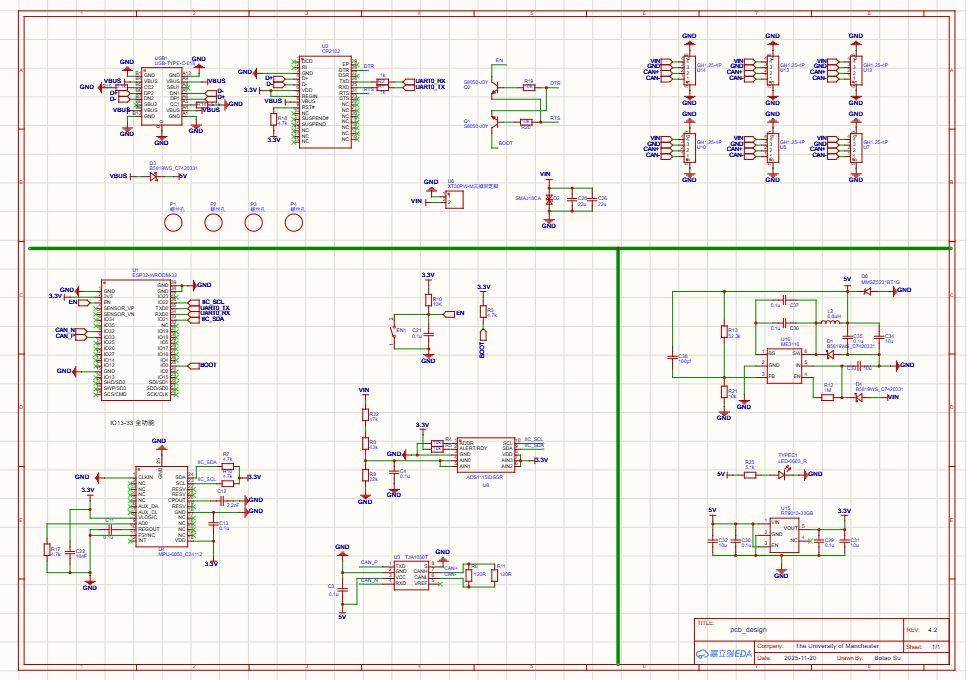
\includegraphics[width=0.92\textwidth]{appendices/Appendix_H_Hardware_and_Control_Evidence/PCB_Schematic.png}
    \caption{自研 ESP32 控制 PCB schematic 导出图。}
    \label{fig:appendix-pcb-schematic}
\end{figure}

\begin{figure}[H]
    \centering
    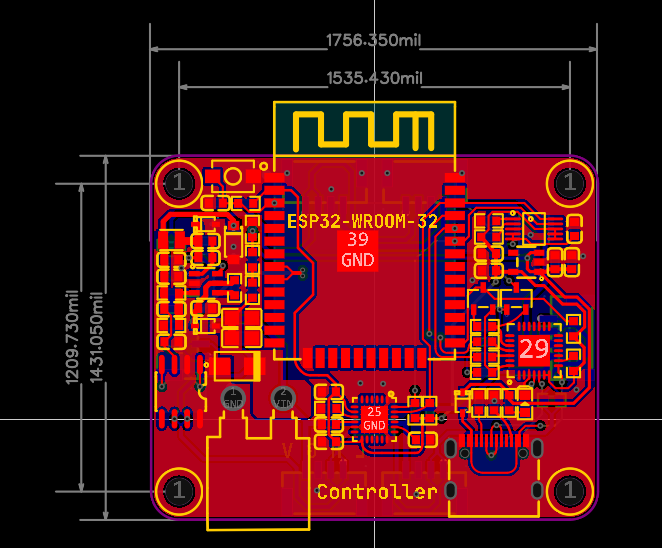
\includegraphics[width=0.84\textwidth]{appendices/Appendix_H_Hardware_and_Control_Evidence/PCB_Layout.png}
    \caption{自研 ESP32 控制 PCB layout 导出图。}
    \label{fig:appendix-pcb-layout}
\end{figure}

动力学和 LQR/VMC PDF 笔记是 Botao Su 的原创项目推导笔记，作为支撑性附录文件保留，不在正文全文复现。

\end{document}
